\documentclass[10pt, a4paper, openany, fleqn,%
               headinclude, footinclude, parskip=half,%
               numbers=noenddot, cleardoublepage=empty]{scrreprt}

\usepackage[utf8]{inputenc}
\usepackage{mathpazo} %-- use Palatino font
\usepackage[left=25mm, top=25mm]{geometry}
\usepackage{amsmath, amssymb, amsthm}
\usepackage[square]{natbib}
\usepackage{subcaption} 
\usepackage{xspace}
\usepackage[breaklinks=true,
            colorlinks=true,
            linktocpage=true,
            allcolors=colorforlinks]{hyperref} 
\usepackage[ruled, vlined, algochapter, linesnumbered]{algorithm2e}
\usepackage{calc}
\usepackage{ccicons} 
\usepackage{xspace} 
\usepackage{longtable}
\usepackage{booktabs} 
\usepackage[english]{babel}  
\usepackage{listings}
\usepackage{scrhack} % ignore warnings about deprecated KOMA-Script
\usepackage[printonlyused, smaller, withpage]{acronym}
\usepackage[usenames, dvipsnames]{xcolor}
\usepackage{graphicx}
\usepackage{pdfpages}
\usepackage{wrapfig}
\usepackage[format=plain, font=small,labelfont=bf]{caption}



\newcommand{\myName}{Céline Dion}
\newcommand{\myTitle}{The optimal Delaunay triangulation of cheesy songs}

\newcommand{\myGroup}{3D geoinformation group}
\def\myGroupLogo{figs/tud-3dgeoinfo-black.png}
\newcommand{\myDepartment}{Department of Urbanism}
\newcommand{\myFaculty}{Faculty of the Built Environment \& Architecture}
\newcommand{\myUni}{Delft University of Technology}

% \newcommand{\myGroup}{Geo-Database Management Centre}
% \def\myGroupLogo{figs/GDMC-LOGO12.jpg}
% \newcommand{\myDepartment}{Department of the OTB}
% \newcommand{\myFaculty}{Faculty of Architecture \& the Built Environment}
% \newcommand{\myUni}{Delft University of Technology}

\newcommand{\myGraduationYear}{2020}
\newcommand{\myGraduationMonth}{February}

\newcommand{\mySupervisorOne}{Prof.dr.\ Jan Smit}
\newcommand{\mySupervisorTwo}{Dr.\ Gerard Joling}
\newcommand{\myCoreader}{ir.\ Gordon Heuckeroth}


%-- for names for \autoref commands
\def\chapterautorefname{Chapter}
\def\sectionautorefname{Section}
\def\subsectionautorefname{Section}
\def\subsubsectionautorefname{Section}
\def\algorithmautorefname{Algorithm}
 
%-- for pdf metadata
\hypersetup{pdfauthor={\myName}}
\hypersetup{pdfkeywords={thesis, geomatics, TU Delft}}
\hypersetup{pdfsubject={A thesis submitted to the Delft University of Technology in partial fulfillment of the requirements for the degree of Master of Science in Geomatics}}
\hypersetup{pdftitle={\myTitle}}

%-- handy shortcuts
\newcommand{\ie}{i.e.}
\newcommand{\eg}{e.g.}

%-- colours for the hyperlinks
\definecolor{colorforlinks}{RGB}{27, 60, 131}




\subject{MSc thesis proposal (P2) in Geomatics}
\title{\myTitle}
\author{\myName}
\date{\myGraduationMonth\xspace\myGraduationYear}
\publishers{A thesis proposal (P2) submitted to the Delft University of Technology in partial fulfillment of the requirements for the degree of Master of Science in Geomatics}

\begin{document}

%******************************************************************
% Frontmatter
%******************************************************************
\frontmatter

\maketitle[3]
%!TEX root = ../thesis.tex

\thispagestyle{empty}

\hfill
\vfill

\noindent\myName: \textit{\myTitle} (\myGraduationYear)\\
\ccby\xspace This work is licensed under a Creative Commons Attribution 4.0 International License. To view a copy of this license, visit \url{http://creativecommons.org/licenses/by/4.0/}.

\vspace{3em}
\vspace{3em}

\noindent{} The work in this thesis was carried out in the:\\

\begin{tabular}{ll}
\parbox{0.3\textwidth}{\includegraphics[width=\linewidth]{\myGroupLogo}}
&
\parbox{0.7\textwidth}
{
  \myGroup\\
  \myDepartment\\
  \myFaculty\\
  \myUni\\
}       
\end{tabular}

\vspace{3em}
\noindent
\begin{tabular}{ll}
Supervisors:  &  \mySupervisorOne \\
              &  \mySupervisorTwo \\
\end{tabular}

%******************************************************************
% Mainmatter
%******************************************************************
\mainmatter

%!TEX root = ../thesis.tex

\chapter{Introduction}
\label{chap:i}

\section{Motivation}
\label{sec:motivation}

Constructing and maintaining an up-to-date graph-like road network on the national level has a range of firmly established uses. Owing to its structure, it can be used efficiently for modelling and simulation purposes, such as traffic flow simulations, passenger transport modelling, construction and upgrade impact modelling (to pinpoint optimal locations and types of investment), and traffic noise load modelling (\cite{bell_lida_1997, zhu_li_2007, zhang_2011, duran_santos_2014, peng_etal_2020}). It can also be used for navigation; a graph-like road network representation is at the heart of most road navigation services (\cite{yue_etal_2008}). Combined with other data sets, we can mention an even wider range of use cases: complemented by ecological statistics and models, it can offer insight into the impact of the presence of roads, and planned road construction on the flora and fauna in their vicinity.

Or to mention a different type of example, an accredited model representing the road network in a digital format may be used as a shared working space when aggregating geospatial data relating to road infrastructure from various sources. It makes it possible for geographical road locations, topographical relationships, and arbitrary semantic information to reside in the same network-type data model, making analysis techniques more straightforward, enforcing consistency and saving effort for data providers who would otherwise all need to maintain their own road model (\cite{ekpenyong_etal_2007}). This example is closely related to the ambitions the provider of the Dutch digital road network, which is the primary subject of this research, has with their road network model.

One may remark that a two-dimensional representation with \textit{approximate} geographical locations may suffice for many of the purposes I listed as examples above, topology being the main concern in network analysis. For instance, \ac{gnss} navigation software often use snapping methods to ensure that the navigating vehicle always traverses the road graph – ensuring that even for imperfect positioning results navigation remains continuous (\cite{fouque_bonnifait_2008, chen_hsu_2020}). Traffic flow simulations are primarily concerned with traffic loads, road properties, and how roads are subdivided by intersections among other aspects. \textit{Mostly}, they are not concerned with the exact geographical locations of roads – as long as the topology is relatively accurate, any geographical permutation of the network will yield largely invariant results (\cite{thomson_richardson_1995}).

However, some applications are concerned with the road network in the context of its surroundings, which makes the accuracy of its georeferencing important. Noise modelling is such an application, because modelling the propagation of road noise concerns deriving the noise load affecting various objects in the vicinity of the the roads. This also involves considering objects that may impact the propagation of the noise, such as noise barriers, terrain, and buildings (\cite{ishiyama_etal_1991, bennett_1997, guarnaccia_quartieri_2012}).

A realistic noise propagation model should take into account terrain, and the 3D geometry of the surrounding objects. It should also take into account the position of roads \textit{relative to the terrain}. For instance, consider a hill with a building on one side and a road on the other, as shown in Figure \ref{fig:justification_illu}. The hill (the terrain) in this case acts as a noise barrier affecting the noise load received by the building. Unless the assumption holds that roads are always found \textit{on} the terrain, this is not yet enough information to derive the noise load. The assumption does not always hold because roads may be elevated, sunken into the ground, or built in tunnels. For instance, if the road in my example is built on a bridge with a similar height as the hill, then the hill will suppress the road noise much less effectively, and "snapping" the road to the terrain by ignoring its elevation would yield incorrect noise modelling results. One way to handle such scenarios is to take into account the absolute elevation of the road surfaces, in other words to use a 3D road network.

\begin{figure}
    \centering
    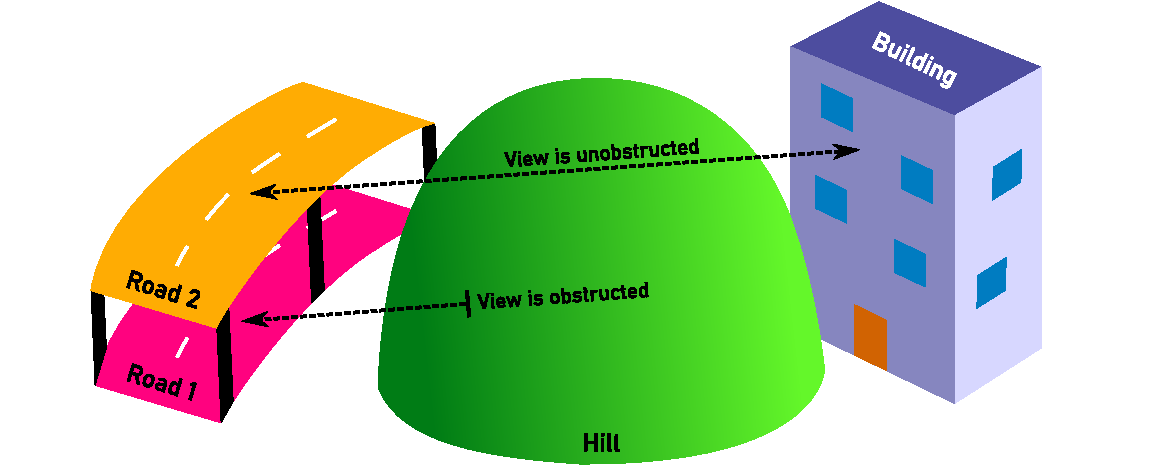
\includegraphics[width=\linewidth]{final_report/figs/justification_illu.pdf}
    \caption[Illustration of the 3D conversion justification]{This illustration shows a justification of the 3D conversion of NWB. Assuming that the road network always lies on the terrain (pink road) allows one to model the propagation of noise with the surrounding terrain and 3D objects taken into account. However, roads above or below the terrain elevation will be represented incorrectly. For instance, the noise from the true location of the road (yellow elevated road) reaches the building. "Snapping" it to the terrain suggests incorrectly that the hill blocks the noise.}
    \label{fig:justification_illu}
\end{figure}

2D-projected digital road models with mediocre accuracy have attracted great scientific and commercial attention since the advent of digital cartography and satellite navigation (\cite{taylor_etal_2001, fouque_bonnifait_2008, yue_etal_2008, chen_hsu_2020}). However, \textit{accurate 3D representations} are still atypical, owing to factors such as increased cost of generation and maintenance, increased complexity of visualisation and analysis, and a lack of significant use cases (\cite{zhu_li_2007, wang_etal_2014}). As a result, 2D road models are common in terms of both public and private geospatial providers, whereas accurate 3D road models are rare in comparison.

When a use case arises and an accurate 3D model is needed, providers generally have two options: to produce a new model, or to enrich an existing 2D model with elevation data. The decision generally depends on the quality of the available 2D data set relative to the requirements for the 3D model, as well as that of the dataset(s) available as sources of elevation data, with which the 2D model can be enriched, among other factors (\cite{zhu_li_2007, zhu_li_2008, wang_etal_2014}). In terms of the source of elevation data, the rule of thumb in the geospatial field is that data acquisition is far more expensive than re-using existing datasets, especially openly available ones. As a result, many providers first attempt to find a way to convert their datasets into 3D using existing data in such a cost-effective manner.

\section{The NDW commission}
\label{sec:commission}

In certain projects the accuracy requirement and restrictions on the modelling procedure may be prescribed legally. Such is the case for the client of the present dissertation research, the \ac{ndw} (National Road Traffic Data Portal), part of \ac{rws} (Directorate-General for Public Works and Water Management), a Dutch government organisation who are in the process of enriching their pre-existing open data 2D road model, called \ac{nwb} (National Road Database), with 3D data, to attain compliance with the new version of the Dutch noise legislation or \textit{geluidwetgeving}, coming into effect on the 1\textsuperscript{st} of January 2022. The new version of the legislation prescribes, among other things, a horizontal \textit{and vertical} accuracy of 20 centimetres for the road model underlying the noise simulations. Due to cost considerations and reasons related to \ac{ndw}’s data acquisition pipeline, the pre-existing 2D version of \ac{nwb} will be converted into a 3D dataset (dubbed \textit{3D-NWB}) primarily using open data geospatial datasets. They have produced a prototype implementation themselves, and subsequently contracted the consultant firm \ac{rhdhv} to create a commercial implementation based on their experience with the prototype. The development of this tool was concluded in December 2020, with a preliminary version of the results already publicly available on their website in addition to the traditional 2D version.

Thus for \ac{ndw}, the next year will be about assessing the quality of their new product and improving it as they see necessary. In particular, they wish to assess how it fares in terms of the requirements set by the law. This dissertation research attempts to contribute to this assessment by presenting an original system design and implementation that favours scientific correctness, and in which output accuracy can be qualitatively and quantitatively examined. By comparing the results of this academic implementation to that of the commercial one, it becomes possible to indirectly evaluate the commercial results' general quality and accuracy in an indirect manner. My work also explores various related geomatics topics in the process, which I specifically refer to as the academic aims of this project, in the present report.

My research was carried out in consultation with the above parties. In fact, the stages leading up to the submission of my dissertation proposal involved continuous consultation with personnel both at \ac{ndw} and \ac{rhdhv} while the commercial implementation was still being developed, to ensure that my research fits well with \ac{ndw}'s plans and the commercial implementation - in addition to answering various questions inspired purely by academic interest.

\section{Field and relevance}
\label{sec:relevance}

For reasons that will later become clear (see Section \ref{sec:input}), I primarily focused on a Lidar point cloud and a 3D topographical line dataset as elevation sources. In both of these datasets, it is clearly evidenced that roads are occasionally in complex three-dimensional relationships with one another and with their environment. For instance, they cross above and below other roads and are also frequently occluded by other objects such as vegetation and buildings. Already in the planning phase of the project the question had arisen, how such real-world geometries should be dealt with in the conversion process - evidently they will require special treatment relative to well-exposed road surfaces. The answer to this question is closely linked with which field of geoscience my project is positioned in.

The likely candidates in the context of digital road network modelling are \ac{gis} and geomatics. It is thus worth discussing briefly how each typically treats 3D objects. One of the reasons why 2D road models are popular is that their geometry and network properties can be analysed using a multitude of well-proven \ac{gis} methods and software kits. However, in \ac{gis} models, even if elevation measurements exist, they are generally only present as an \textit{elevation attribute} (i.e. a semantic data field, like street names), because \ac{gis} geometrical models do not typically support true 3D operations. This is conceptually identical to projecting the geometries onto the horizontal plane. Geometric models that treat the vertical dimension explicitly are more common in geomatics; namely 2.5D and 3D models. While using 2.5D models restricts the types of physical entities that can be modelled, it also greatly simplifies certain types of analysis conceptually and computationally. This makes it ideal for working on similar scales to \ac{gis}; on the national scale for instance, as in this research.

While 2.5D modelling initially appears to be a good candidate for this project, we may observe that it is by definition unsuitable for handling the 3D relationships that roads have with each other and with their environment. However, much like how the concept of divide-and-conquer works in computer science, it is also possible decompose three-dimensional, geometrical problems into smaller sub-problems until they become natively compatible with 2.5D methods which are simpler to solve individually than the 3D problem as a whole. This research is positioned in the field of geomatics because my system design is specifically intended to explore how 2.5D methods can be applied in a way that enables the \textit{piecewise} modelling of a national road network. The divide-and-conqer concept will be applied to decompose the road network into segments that can be individually, locally regarded as \textit{terrain} (i.e. a mathematical surface) and hence be modelled in 2.5D.

Geomatics is comprised of a wide range of disciplines, several of which are relevant to the present research. As it focuses on 2.5D methods to a great extent, it overlaps with the geomatics field of \textit{digital terrain modelling} in terms of how it generates and stores the digital representation of road surfaces, and as a consequence, the manner in which it will derive elevations from them: using \textit{spatial interpolation}. As the overview of the methods in Section \ref{sec:methodsoverview} reveals, it also strongly overlaps with the geomatics discipline of \textit{feature extraction} (and to a lesser extent, \textit{photogrammetry}), because of the intermediate steps used by the pipeline to derive the 2.5D road surface models from our input datasets.

This is in line with my goal to study how a combination of mainly geomatics-based tools and methods can be used to accomplish the tasks required by \ac{ndw}, and to also assess their accuracy and suitability when used in this way. However, I also use \ac{gis} methods "under the hood" in all parts of the project - for instance, 2D geometry intersection tests, orientation tests and spatial queries are pervasive in the implementation, and are thus often mentioned in the detailed description of the processing steps found in Section \ref{sec:methods}. Furthermore, my research often touches on mathematics and statistics, for instance I use polynomial fitting and maximum likelihood estimation (\ac{mle}) throughout the implementation (as examples of the former) and metrics such as standard deviation and \ac{rmse} (as examples of the latter).

\section{Research questions}
\label{sec:rq}

My main research question is \textit{"How can we achieve a 3D conversion of the \ac{nwb} dataset using Dutch open geospatial data and a primarily 2.5D-based surface modelling methodology, while guaranteeing optimal and quantifiable accuracy and completeness?"}. It was distilled from the main areas of interest that we settled on during the preparatory stages of the project, while planning the project with my academic mentors, as well as \ac{ndw} and \ac{rhdhv}. The question is comprised of two halves, which I initially intended to devote equal amounts of attention to - the question of devising a system design and implementing it, and that of assessing its effectiveness and the accuracy and completeness of the output it generates (as well as comparing it with the commercial results).

I eventually settled on focusing more time and effort on the system design and integration (i.e. \textit{performing} the elevation-enrichment of NWB), both because it required more time than initially anticipated, and because the quality and accuracy assessment of the results (and their comparison with the commercial results) was more straightforward than expected. Furthermore, I found that many of the accuracy-related questions depend strongly on the exact specifications of the system design and its implementation, meaning that not all the work necessary to answer those questions was clearly separated into a dedicated accuracy assessment process - much of it needed to be considered and evaluated during the development process.

The two halves of the main research question were created by collecting my sub-questions into these two categories; pipeline design and implementation, and accuracy assessment. Below I present some of these sub-questions, to characterise in somewhat more detail, what specifically my attention was directed towards in this research project. 

\begin{enumerate}
    \item Sub-questions related to \textit{performing} the elevation-enrichment of \ac{nwb} using Dutch open geospatial data and predominantly via 2.5D geomatics methods
    \begin{enumerate}
        \item What are the exact methods of the commercial implementation and what do we suspect its theoretical shortcomings to be?
        \item Does the literature suggest any methods that are particularly suitable to this research? If so, can we make use of them in our own methods?
        \item How can the academic methods best make use of the combined information content of the datasets that the commercial implementation uses?
        \item How should the road network be subdivided into parts that each represent a 2.5D problem? Can they be processed individually to facilitate easy parallel processing?
        \item As we are using Lidar data, can we produce an accurate and complete \ac{tin} surface model for each 2.5D "unit"? Can we interpolate elevations for \ac{nwb} through this model?
        \item How do we "stitch" the results of the individual 2.5D procedures back together into a 3D road network with the correct topology?
        \item Can the implementation be made robust enough to handle all (or \textit{most}) challenging road layouts correctly, such as complex motorway junctions?
        \item How can we make the implementation perform well in areas where input elevation data is scarce or missing over longer distances, such as in tunnels?
        \item Can the computational complexity of the program be kept low enough to be suitable for processing all the relevant roads?
        \item While solving \ac{ndw}'s specific problem, can we also ensure that our solution generalises well to other problems of a similar type?
    \end{enumerate}
    \item Sub-questions related to the \textit{assessment} of the overall quality, completeness and accuracy of the output and its similarity to the commercial results
    \begin{enumerate}
        \item In related work, what methods are typically used to measure empirical and theoretical output accuracy?
        \item According to related work, what typically defines output accuracy? Do local factors also play a role, or is it reasonable to estimate it for the procedure globally?
        \item What is the accuracy of our input elevation data sources? Can we structure the pipeline in a way that their input accuracy can be propagated to the output in a straightforward manner?
        \item To facilitate the above, can we derive our output directly from input data points, despite the large number of processing steps that are potentially necessary?
        \item What is the effect of uncertainty in the lateral positions of \ac{nwb} centrelines on the effectiveness of our methods, and on the output accuracy?
        \item The road surface model \ac{tin}s are also important products of the pipeline. How can we assess the overall quality and completeness of these?
        \item Can we indicate it in the output, which input elevation source each output elevation estimate was derived from, and to use this capability to derive the output accuracy from the appropriate input dataset's accuracy?
        \item How are temporal inconsistencies between the datasets manifested in the output? Can these be detected by the processing steps?
        \item In case we can estimate accuracy on the local scale, what physical features or sensing issues do drops in accuracy correspond to? If this corresponds to problems with the input, what properties of the input should be improved?
        \item How good is the agreement between the commercial and the academic results? What physical features or sensing issues do disagreement between the results correspond to?
        \item Under what conditions does the academic solution perform better or worse than the commercial one, and what does this tell us about the two underlying sets of methods?
    \end{enumerate}
\end{enumerate}
%!TEX root = thesis_proposal.tex

\chapter{Research questions}
\label{chap:rq}

The decision was made to include the research questions before the Related work section. The justification for this change is that in this particular research, the research questions primarily emerged from the requirements of the NDW assignment and the suspected shortcomings of the commercial implementation. The literature review was \textit{targeted} at identifying a range of methods that could be used to complete the 3D enrichment of NDW while ensuring and quantifying output accuracy and resolving the suspected issues with the commercial implementation. The research questions are presented as a range of primary questions along with secondary sub-questions.


\begin{enumerate}
\item Is it possible to find a combination of geomatics methods that can perform the elevation-enrichment of NWB in a similar manner to the commercial implementation, but eliminating suspected shortcomings as best as possible?
\begin{enumerate}
    \item Can this be done using the same (or equivalent) datasets as the ones used in the commercial implementation?
    \item Is the existing accuracy of NWB itself good enough to support such a workflow?
    \item Is it possible to based the workflow entirely on 2.5D methods by decomposing this intrinsically 3D problem into a collection of smaller problems?
    \item Can such a method of decomposition be used to simultaneously solve the scaling issues related to handling a national Lidar paint cloud input dataset?
    \item Is it possible to build a workflow that satisfies the above, but also allows efficient updated operations to be carried out as new data arrives or old data is updated?
    \item Benchmark the solution in areas of complex 3D relationships and optimise the implementation accordingly.
    \item Benchmark the solution in areas where input data is scarce due to occlusion or other reasons and optimise the implementation accordingly.
    \item Explore whether lines representing the vicinity of the roads can be enriched with elevations in the same way.
\end{enumerate}
\item 
\begin{enumerate}
\item Research and assess the initial accuracy of the input datasets. This includes NWB itself.
\item Track changes in accuracy throughout the procedure
\end{enumerate}
\end{enumerate}
%!TEX root = thesis.tex

\chapter{Related work}
\label{chap:rw}

I found and studied a large number of research papers as part of the literature review stage of this project. When I started the review, I already had a good starting point on what specifically to research, because had known that my focus would be restricted to three specific, openly available Dutch geospatial datasets, and because I had already settled on a range of specifics regarding the goals and requirements of the project. The three datasets were picked early on in the planning process for reasons related to our wish to mainly use the same datasets as the commercial solution does.

As it is the most up-to-date detailed elevation source, and thus suitable for performing detailed surface modelling in addition to the 3D conversion of lines, my primary candidate became the national ALS point cloud of The Netherlands. The name of the latest release of this product is abbreviated AHN3. As a result of this choice, there are two main areas that I focused on as part of my literature review: road feature reconstruction from Lidar point clouds, and the theoretical and empirical propagation of Lidar accuracy into derived models. The literature review concerning these two areas is presented below in two independent parts.

The other two datasets are NWB itself, and a 3D line dataset called DTB which has coverage in many areas where AHN3 does not. Detailed information about the choices regarding the datasets, as well as an analysis about their detailed properties, can be found in in Section \ref{sec:input}.

\section{Road identification in point clouds}
\label{sec:roadidentification}

My main domain of interest was feature extraction from Lidar data, because tasks of this type characterised the bulk of the planned processing pipeline. Our intention was to not only query a DEM for elevations around the NWB road centrelines - an example of a simple way in which one could perform a \textit{rudimentary} 3D conversion - but to create spatial models of road edges and surfaces, and only then proceed to extracting elevations for the centrelines. This requires one to identify, or at least approximate the geometries of these features by choosing the point cloud points that best describe them and applying various operations to them.

We may thus regard point cloud feature extraction as the top-level geomatics topic concerned by this research, with most other operations, such as 2.5D surface modelling and mathemamatical tools, as residing a level lower in the hierarchy. We are using them for the purpose of identifyng and modelling discrete physical features found in the point cloud (and the support dataset, which will be discussed later in this chapter).

\subsection{Research using point clouds only}
\label{sub:roadidentification_pconly}

\subsubsection{Approaches based on photogrammetry}

In terms of point cloud feature extraction techniques relevant to roads specifically, I studied a range of papers detailing a wide spectrum of methods. One strategy, most prominently represented by \cite{hu_2003, hu_etal_2004, zhu_mordohai_2009, zhu_hyppa_2014, lin_etal_2015}, is based on the idea of transitioning to a photogrammetric analysis at some point in the process, generally quite early on. First, a set of pre-processing techniques to better characterise potential road points in the source Lidar data are applied, generally by performing some form of filtering (e.g. setting intensity thresholds applicable to Lidar returns from bitumen), or by extracting ground planes using various techniques and selecting points that lie close to them. Then, images are rendered from the point cloud from various angles, often using colour-coding based on point properties, and applying photogrammetric methods to identify roads. Sometimes, high-definition aerial or satellite imagery is incorporated in the photogrammetric workflows. The success rates of such strategies are mediocre, and they rely strongly on manual parametrisation. In particular, they are unsuitable for large study areas with inhomogeneous types and distributions of roads, as also concluded by the excellent review of this type of relevant work in the literature review section of the paper \cite{yang_etal_2013}.

\subsubsection{Approaches based on curb detection}

A further popular set of strategies rely on road curb detection. \cite{vosselman_zhou_2009}, \cite{zhang_2010}, and \cite{yang_etal_2013} are examples of such research. \cite{vosselman_zhou_2009} presents a method in which a DTM is generated, points close to its surface are selected from the point cloud and small, curb-like jumps in elevation are algorithmically detected using thresholds. The curb points are selected, and a feature extraction method (RANSAC in this case) is used to construct 3D lines from them. Gaps in the lines are closed procedurally, and B-splines are fitted to optimise the shapes of the road edges. In \cite{zhang_2010}, road cross-sections are constructed and inspected in 1D, and points are "classified" based on whether they are likely to represent road surfaces, curbs, or off-road surfaces. To do this, they process MLS data on-the-fly (during acquisition) via a supervised classifier, and use the Hough transform to model the road surface. The curbs are found where the points first deviate from the model.

In \cite{yang_etal_2013} a similar approach is presented in which cross-sections are identified by looking at MLS scan properties (time of acquisition, specifically), and then non-road points are filtered out in 1D based on the absolute elevation of the road (known from constant elevation of the sensor above it) and curbs \textit{of a specific type} are identified in the 1D series of ground points - all via a single moving-window operation that uses applicable thresholds.

While the results of the curb detection-based methods are more flexible, more accurate and more complete in general than the photogrammetric methods, they are not well suited for my project out-of-the box. These approaches work best with MLS data, where the data is either natively produced in the form of road cross-sections (the scan lines of a car-mounted front facing sensor), or can be easily extracted from the point cloud in such a form. Furthermore, in MLS sensing the road elevation is generally known, by considering the sensor's constant position relative to the vehicle's GNSS sensor - this is not the case in ALS. Lastly, while the above method may work well in places where curbs are well-defined, this is not a reasonable assumption to make for an ALS dataset with nationwide coverage, such as our particular input.

The work \cite{vosselman_zhou_2009} is not entirely bound by the above limitations. It demonstrates that a relatively simple approach can be used to detect curbs without the need for the point cloud to be comprised natively of cross-sections, and for accurate road elevations to already exist. However, the fact that it also uses curb detection with fixed thresholds undermines my confidence in it. Working with a national dataset and focusing on large roads (including motorways, one of our main targets for 3D conversion) means that the assumption that well-defined, relatively uniform road curbs will exist and be reliably detectable everywhere is not a sensible assumption.

\subsubsection{Other, purely Lidar-based approaches}

There are many other papers that deal with this task without relying on external vector data. For instance, \cite{clode_etal_2004} and \cite{clode_etal_2007} present a set of methods in which first a DTM is generated, then points close to the DTM are selected and are further filtered based on intensity and sampling density thresholds applicable to reflections from flat bitumen surfaces. The results are converted to a raster mask which is then refined via morphological operations. It is then used to produce the output: a point cloud in which road points are marked semantically (i.e. they are classified as such). In the 2007 paper, they extended the procedure by convolving the results with a Phase Coded Disk (PCD), which can create a 2D map of the predicted road parameters wherever it moves through road points. Like the morphological operations above, the PCD-convolution is in fact a photogrammetric method, because it also acts on a raster generated from the classified point cloud prior to its application. Nevertheless, the method is still more relevant to us than the rest of the photogrammetry-based research mentioned here. An example visualisation of its output is shown in Figure \ref{fig:phasecodeddisk}, the vector magnitude in any given pixel quantifies the support that exists there for the presence of a road centreline - it is effectively a centreline detector. They describe it as an alternative to using the Hough-transform for finding road centrelines, which, according to their research, is not reliable enough in this context. This spatial map can then be used to generate a vector dataset describing the geometry of the roads.

\begin{wrapfigure}[20]{O}{0.48\linewidth}
    
\includegraphics[width=\linewidth]{final_report/figs/clode_etal_2007_01.png} 
    \caption{Illustration of the results of PCD convolution from \cite{clode_etal_2007}.}
    \label{fig:phasecodeddisk}
\end{wrapfigure}

The research \cite{gross_thoennessen_2006} shows that point neighbourhood information can be used to generate covariance matrices of individual points, which can in turn be used directly to indicate if the point belongs to a linear feature. They also describe how lines can be assembled from the selected points efficiently. Although their methods have very well documented mathematical foundations which could be reproduced in any programming language, their applicability in my research, especially in the context of small or even non-existent curbs, is uncertain.

Other methods relying purely on the Lidar points themselves exist, but like \cite{zhang_2010}, they are typically intended for real-time MLS applications - such as the fully convolutional neural network-based solution in \cite{caltagirone_etal_2017}. The literature review in \cite{yang_etal_2013} offers an excellent overview of such additional methods, but they will not be described here any further, as I found them not to be relevant to this project.

\subsection{Research using input point clouds and approximate road locations}
\label{sub:lidaraccuracy_external}

This section contains brief descriptions of research that used similar input data to mine \textit{in addition to} Lidar data; mainly vector datasets estimating road centreline positions. These relevant papers describe work that used analogous input data to achieve similar goals to mine - as a result, they contain the methods that are the most relevant to my own research.

\subsubsection{Relatively simple approaches}

The work \cite{hatger_brenner_2003} presents two approaches based on region-growing. The first one is based on growing planes in the entire study area from Lidar points. Finding this to be too complex computationally, they propose another approach of treating Lidar scan lines individually, partitioning each into parametrised line segments via linear regression and then inspecting the succession of scan lines and identifying neighbouring segments that are roughly parallel. The resulting groups of (roughly parallel) 3D lines are then treated as cross-sections of planar regions, and an additional region growing step is performed to find any points that might have been left out in the previous steps. The results of this can then either be prepared as a full, 3D planar partition of the study area onto which road polylines can simply be projected, or they can be further refined first by eliminating small, meaningless planes via a RANSAC-based workflow.

The work \cite{cai_rasdorf_2008} shows that enriching road centrelines with elevations can be achieved using even more simplistic methods. Their first method is based on finding points on opposite sides of roads (in 2D) at similar distances from them, and in suitable locations to form approximate cross-sections. The centrelines are intersected with the cross-sections and are given elevations at the points of intersection. The elevations are computed by interpolating linearly inside the cross-sections, using the elevations of the two points that define each of them. Their second method is even simpler; for each road vertex  (or some sampling along its length), they locate the closest Lidar point and associate its elevation with it. The simplicity of these methods is reminiscent of the NDW prototype and the commercial solution developed for NDW by RHDHV (described in Section \ref{sec:methodsexisting}), and highlights that a rough approximation for the road elevations can, in practice, be made either directly from the point cloud or from a derived DTM in a straightforward manner. However, far more sophisticated methods have been developed by other authors.

\subsubsection{Complex approaches based on active contour optimisation}

One landmark paper, \cite{boyko_funkhauser_2011}, describes a method in which a set of 2D input LineStrings are used to identify and label road points in an ALS point cloud. The input lines contain road intersection nodes and patches, from which centrelines are derived. They first associate the input lines with elevations by fitting spline curves through Lidar points close to the centrelines in 2D. Suitable Lidar points are selected by minimising an error function that includes terms related to the distance from the location of interpolation, and to elevation variance. The resulting network is guaranteed to be continuous and smooth because the densified input polylines are used as spline control points. Since the entire system of splines is connected, this is also guaranteed to minimise the effects of local issues, such as occlusion.

\begin{figure}
    \centering
    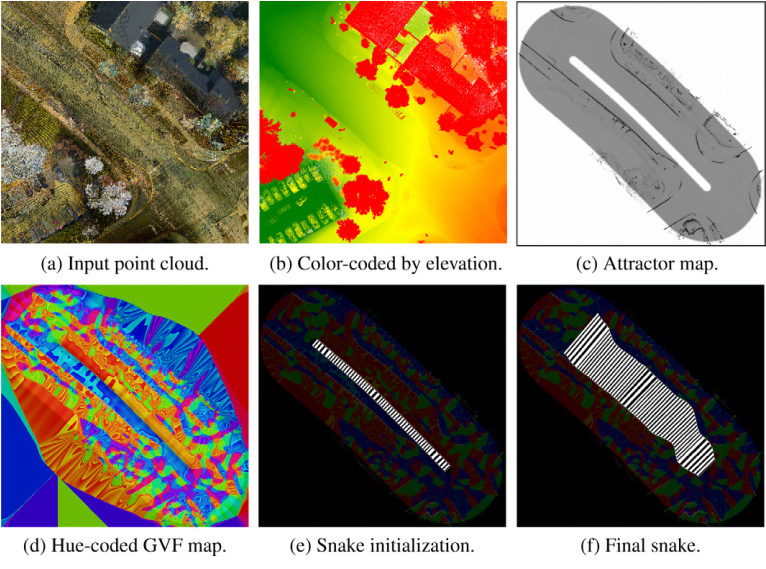
\includegraphics[width=0.85\linewidth]{final_report/figs/boyko_funkahuser_2011_01.png} 
    \caption{Illustration of the contour optimisation procedure used in \cite{boyko_funkhauser_2011}.}
    \label{fig:boykofunkhauser2011}
\end{figure}

The point cloud is then partitioned on disk, based on fitting support planes along the 3D-converted lines and fetching points that are close to them, solving performance-related issues of working with too many Lidar points at once, and further minimising the effects of 2.5D violations related to overlapping features. They then construct scalar maps for each resulting segment that penalises points away from road edges (both inwards and outwards). These maps, called attractor maps, are composited from rasters penalising locations that are outside the range in which edges are expected to be found (relative to the centrelines), and rasters produced by a curb detection metric related to the normal vectors of the point cloud points. Lastly, they apply an active contour optimisation technique (specifically, ribbon snakes) that yields the road edges in 3D, and then labels points between the two edges as road points. An illustration is shown in Figure \ref{fig:boykofunkhauser2011}, taken from their paper. In the attractor map, darker colours represent stronger attraction, resulting in the active contour converging to them in the optimisation procedure. The GVF map is a vector map that contributes to favourable active contour convergence and is not described any further here (please refer to the original paper). The initial contour is based on the road centreline (from external vector data).

The results of \cite{gopfert_etal_2011} demonstrate that active contour optimisation can be used to estimate road outlines without the need for the involved pre-processing steps of \cite{boyko_funkhauser_2011}. They convert the input point cloud directly into a DTM, and then into attractor maps. They use the same general type of active contour optimisation, and generate output centrelines and road edges with comparable quality to that of the outputs of \cite{boyko_funkhauser_2011}. It is worth mentioning that the type of active contour optimisation used by these two papers also optimises the road centrelines in conjunction with the road edges, which is particularly important in places where the 2D georeferencing of the original centrelines is poor.

\subsubsection{Relevant work with Dutch data}

The work \cite{oudeElberink_vosselman_2006} is relevant not only because of the methods it applies, but also the specific datasets. They enrich the best-known Dutch open data national topographical vector dataset (the present-day equivalent of which is BGT) with elevations, and as their source of elevations, they use AHN data (the first edition of AHN, the third edition of which I used in my own research).

\begin{wrapfigure}{O}{0.5\textwidth}
    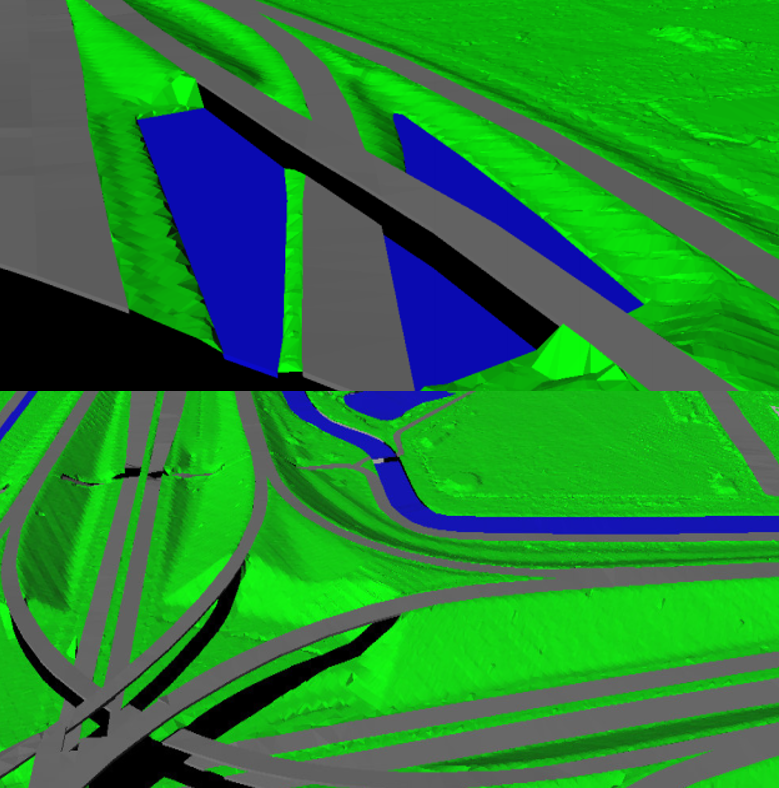
\includegraphics[width=\linewidth]{final_report/figs/oudeElberink_vosselman_2006_03.png} 
    \caption{Examples of 3D-converted multi-level road vector geometry from \cite{oudeElberink_vosselman_2006}.}
    \label{fig:conversionartefacts}
\end{wrapfigure}

They do not exclusively consider roads; all polygonal vector objects are extruded to 3D. Like in \cite{hatger_brenner_2003}, a region growing approach is proposed as the foundation of the elevation extraction workflow. They use the Hough transform to find seed points whose neighbourhood suggests a planar structure, fit planes and then grow them by checking the point-to-plane distance of new points, labelling points with the identifier of the plane they belong to. The vector data is then overlain on these regions and for each polygon, the plane is selected which is represented by the greatest number of labelled points in its interior. These points are re-fitted a plane, and each such plane is used to extrude the corresponding overlain vector geometry simply by projecting the polygon onto its surface. To improve upon the results of this simple extrusion, they suggest the application of algorithmic topological corrections. Furthermore, to model the interior of the extruded polygons in more detail, they recommend the construction of a Constrained Delaunay Triangulation (CDT) for each, first by inserting its edges as constraints, and then by inserting the Lidar points that its surface is based on. The CDT can be refined procedurally to ensure smoothness. The main limitations of their methods are that the extracted elevations (from the region growing approach) are not reliably accurate, and that it cannot handle overlapping objects, such as roads in motorway interchanges. 3D visualisations of the results of this approach and typical artefacts are shown in \ref{fig:conversionartefacts}. The specific artefacts shown in the figure demonstrate that in multi-level road layouts, only the topmost road is fully converted to 3D.

Their method was later extended in \cite{oudeElberink_vosselman_2009} to work well in complex multi-level road settings by using point cloud segmentation in a manner resembling what I already described in the context of \cite{boyko_funkhauser_2011}, which we may regard in general as decomposing the 3D problem into 2.5D sub-problems, also a main aim of my own research. In his doctoral thesis \cite{oudeElberink_2010} he combined this method with the overall procedure in \cite{oudeElberink_vosselman_2006} to form one integral whole. Furthermore he extended it with a road extraction quality and accuracy assessment procedure, which was later perfected and also published separately in \cite{oudeElberink_vosselman_2012}.

Their quality and accuracy assessment methodology is comprised of two separate procedures and the comparison of their results: a theoretical (error propagation-based) evaluation, and an empirical one against reference data. Their error propagation-based evaluation takes into account metrics such as GPS and INS noise in the Lidar survey (suggesting that they had access to low-level information about the dataset), plane fit quality and observed Lidar noise. It also considers interpolation/extrapolation uncertainty, relevant in places where not enough relevant Lidar points could be located and thus such gap-filling measures were used. They found that these theoretical errors were generally below 20 cm, with noticeable increases only occurring where Lidar coverage was extremely sparse or non-existent, leading to the necessity of using interpolation or extrapolation. 

Interestingly, their reference data was DTB for the empirical evaluation of accuracy, which is also the support dataset I used in my research (see Section \ref{sub:dtb}). In general, their comparison with DTB showed good agreement with their road surface extraction results, except for the same places where the theoretical approach also suggested large errors, and in particular in places where this was also combined with intense vertical road curvature locally, which DTB managed to capture, but not their results. In places with good Laser coverage, the agreement was much better, often near-perfect. Although not explicitly mentioned, it appears that they still used the earliest version of AHN (not AHN2) in this research, which may explain how it is possible that they encountered low point densities even in well-exposed road segments. AHN2 and AHN3 no longer have this problem, as mentioned in \ref{sub:ahn} and in many other subsequent parts of this report.

\subsubsection{On using a support dataset in addition to Lidar data}

In Section \ref{sec:input} in this chapter, I discuss that this research is also concerned with  another source of elevations, which I often refer to as the "support dataset" in this report because AHN3 is given priority to in the analysis, wherever it exists. It is a 3D line dataset, not an ALS or MLS point cloud. The one area \textit{not} explicitly covered in any of the papers I examined is the use of such external 3D vector data as a further constraint when extracting road elevations and/or geometries from point clouds.

In relevant work, occlusion is generally accepted to represent gaps in coverage, and elevations are simply interpolated or extrapolated inside them if possible - or if not, they are not considered any further. In the case of my research, NDW is interested in producing a 3D conversion of NWB with the highest possible \textit{completeness}. Exploring how information from the two datasets can be combined is also interesting academically, thus my work will examine how DTB can be used to patch in gaps in AHN3 coverage. While doing so, I will be building solely on my own ideas, as I could not find work that is directly relevant to this topic.

\section{Lidar accuracy and sampling density}
\label{sec:lidaraccuracy}

Relevant aspects of Lidar-related accuracy assessment can be divided into two main sub-topics: interpreting the reported global and/or local accuracy and areal sampling density of the Lidar surveys themselves, and assessing the accuracy of digital terrain models (DTMs) that one may derive from Lidar point clouds, and the elevations that can be interpolated from them. Although some of the relevant work I studied overlaps with both of these areas, I separated the discussion below into two sections based on them. As Lidar sensing accuracy and sampling density underlies that of the derived models, I discuss it first below.

\subsection{Accuracy description of Lidar sensing}
\label{sub:lidaraccuracy_sensing}

\subsubsection{Global and local influences on accuracy}

\begin{wrapfigure}{O}{0.46\textwidth}
    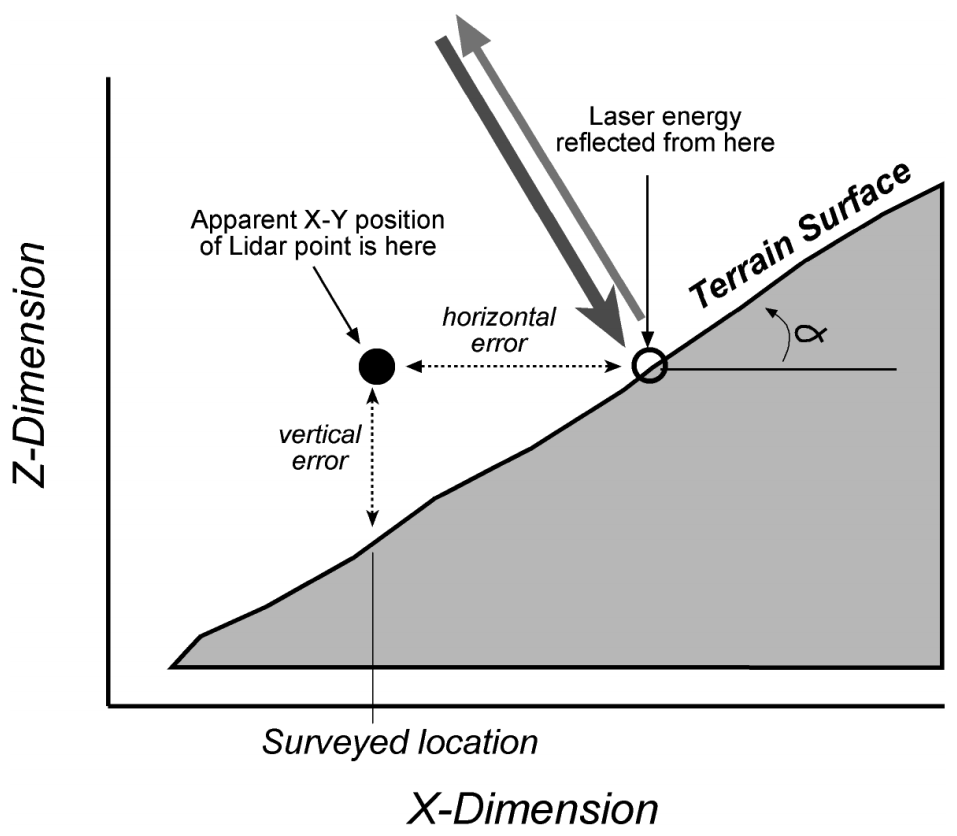
\includegraphics[width=0.95\linewidth]{final_report/figs/hodgson_breshanan_2004_01.png} 
    \caption{Illustration of the effects of terrain slope on vertical accuracy from \cite{hodgson_breshanan_2004}.}
    \label{fig:elevationaccuracy}
\end{wrapfigure}

Many papers describe that the accuracy of Lidar-derived DTMs depends primarily on the accuracy of the sensing method itself. The notable paper \cite{hodgson_breshanan_2004} describes the most fundamental sensing errors of Lidar measurements to be introduced by Global Navigation Satellite System (GNSS, such as GPS) errors, Inertial Navigation Unit (INS) errors, Inertial Measurement Unit (IMU) errors, errors introduced by the waveform analysis algorithm and lastly, a general error factor that depends on the flying height. Combined, these are the primary factors that contribute to the \textit{measurement} accuracy of the sensing system.

It is shown by various papers including \cite{hodgson_breshanan_2004, su_bork_2006, kraus_etal_2006, raber_etal_2007, peng_shih_2006, chow_hodgson_2009, aguilar_etal_2005, aguilar_etal_2010, guo_etal_2010} that there are local factors influencing \textit{vertical} Lidar accuracy that are independent of the sensing equipment, and thus vary from survey to survey. In production datasets, whether they are considered at all or not, they are almost never \textit{reported} locally, i.e. on the level of individual measurements. This is mainly because they are difficult to estimate without a complex analysis of the measured data and potentially, that of external data. Unless the global errors reported in the survey's specifications were derived empirically (e.g. by using ground control points), the effects of local factors specific to the survey may not be reflected in them at all, and they can be considered purely theoretical sensing-related values.

\subsubsection{What influences measurement accuracy locally?}

First and foremost, local accuracy depends on the inclination of the surveyed terrain at the point where the Lidar reflection occurred, as shown in Figure \ref{fig:elevationaccuracy}. Any uncertainty in the lateral position of the point of reflection will be scaled by the tangent of the slope angle, denoted by $\alpha$. The vertical error thus increases linearly as a function of increasing slope (commonly derived from a 2D slope map). Therefore, if the accuracy of a Lidar survey was derived empirically, it will indicate higher errors than the sensing equipment's specifications would suggest, in survey areas with considerable relief.

Elevation accuracy also depends on the vegetation encountered. In all cases, the presence of vegetation decreases it, with the significance of the error depending strongly on the type of vegetation. Mature trees and evergreens tend to influence accuracy to a lesser extent, whereas bushes, shrubs and undergrowth in general tend to have a decidedly larger impact. \cite{peng_shih_2006} quantified this as a function of \textit{vegetation angle}, a qualitative metric that describes how "open" certain types of vegetation are to Lidar. They found that there is a linear correlation between elevation errors and vegetation angle, as well as canopy volume. The one exception I found is \cite{raber_etal_2007} which reported specifically that in very strongly vegetated areas, no correlation could be found between vegetation classes and accuracy (or even point density and accuracy). Still, the majority of relevant research indicates that Lidar accuracy reflects the extent and type of vegetation coverage in addition to its dependence on the relief of the surveyed terrain.

Both the official quantification of measurement accuracy and research tackling these topics often uses empirical methods. They generally consist of surveying ground control points accurately and either directly comparing these with nearby Lidar points, or first constructing a spatially continuous DEM and comparing the DEM-interpolated elevations with the surveyed reference elevations, with the latter approach being more relevant to the next section. The global value is usually specified as the measurement error (in metres or centimetres) at one or two standard deviations, with separate values given for horizontal and vertical errors. The two errors differ in terms of the equipment influencing them, and also because the local factors I outlined above affect elevation accuracy only (as a \textit{function of} horizontal accuracy in the case of local terrain slope). They are generally reported as one or two standard deviations, corresponding to 68\% or 95\% confidence, in metres or centimetres.

\subsubsection{Sampling density as a survey property}

Sampling density describes how many reflections the sensor records per unit area. This is the third descriptor that is commonly found in the documentation of Lidar datasets, and like vertical and horizontal accuracy, it is generally represented by a single global value. This, too, fluctuates locally, and in this case anything between zero and the maximum nominal value of the survey's sampling density is possible. The maximum possible value depends on the sensing equipment and the number of times any given area is scanned (the number of passes). Sampling density does not directly affect the accuracy of individual Lidar measurements, which is one of the reasons why it is reported separately - its effects are more relevant to the next section.

Sampling density is mostly reported as the mean number of points per square metres found in the dataset, occasionally as a range if one or two standard deviations are taken into account. It can be derived from the data directly, i.e. it needs no additional processing or surveying. Relevant studies report that sampling density varies mostly as a factor of terrain relief, vegetation cover, and vegetation angle, with increases in any of these factors resulting in decreases in local point density. For instance, sampling density falls off logarithmically with increasing terrain slope (\cite{peng_shih_2006}, \cite{chow_hodgson_2009}).

\subsection{Accuracy description of Lidar-derived DTMs}
\label{sub:lidaraccuracy_dem}

\subsubsection{Spatial interpolation in the context of DTMs}

In practice, the quality and accuracy of Lidar-derived DTMs is most commonly evaluated via sampling their surfaces to serve as the basis for comparisons. Sampling a DTM takes place via spatial interpolation. The DTM's relationship with the raw data can be established by interpolating at the horizontal locations of Lidar points, while that with the real-world terrain can be examined via surveying control points and interpolating at their 2D positions in the DTM. Intuitively, DTMs provide a link between ground control points and Lidar measurements, which in turn also provides a convenient interface for evaluating Lidar survey accuracy empirically (as I mentioned in the previous section), provided that interpolator's effects on accuracy are known.

Raster DTMs are themselves produced via spatial interpolation. One may convert a Lidar point cloud into a TIN-based DTM without interpolation (the TIN vertices will be Lidar points), but to create a raster DTM, one will need to use a suitable interpolator, such as Inverse Distance Weighing (IDW). Alternatively, a TIN-based DTM can be constructed as an intermediate model and the raster can be derived from it via applying a TIN-based spatial interpolator, such as the Laplace interpolator. These observations entail that a comparison between the Lidar points and their TIN-interpolated counterparts would yield no residuals, i.e. TIN models do not lose information relative to the \textit{ground reflections} found in the Lidar data.

\subsubsection{Evaluating interpolation accuracy}

Spatial interpolators do not leave accuracy unchanged, which cannot be neglected when performing the above benchmarks. For us in this research, the effect interpolators have on accuracy is particularly interesting because the final NWB elevations are produced via spatial interpolation in a Lidar-derived DTM. There exist various approaches to establishing the nature of the relationship between input and output accuracy, such as deriving exact error propagation formulae from the mathematical descriptions of interpolators, as well as the more popular empirical approaches based on \textit{testing} accuracy post-interpolation via split-sample, cross-validation or jack-knife methods. Theoretically, input accuracy (survey accuracy) and any necessary metrics of local influences can then simply be plugged into the formula to obtain the local accuracy post-interpolation.

\subsubsection{Propagating local factors through interpolation}

However, we know from the previous section that the survey accuracy is \textit{itself} influenced by local factors. Since only global accuracy values generally exist for Lidar surveys, the theoretical or empirical error propagation formula may need to be extended with additional terms approximating the influence of these additional factors, depending on how accurately one wishes to approximate output accuracy. The exact nature of this part of the relationship depends on the fundamental principles I outlined in the previous section, and it too, can be modelled both theoretically and empirically. Theoretical approaches are more common for simple relationships (such as that with local slope, as shown in Figure \ref{fig:elevationaccuracy}), while empirical ones are almost always employed in more complex ones (such as the relationship with vegetation). In the context of digital terrain modelling, there is an additional factor we need to consider: ground filtering accuracy. While we wish to model the terrain surface only, the raw Lidar data includes non-terrain reflections that need to be removed before constructing the DTM. This accuracy is also generally estimated, rather than derived theoretically. It is also possible to try to derive the combined effects of all these factors at once, e.g. via Monte Carlo simulations.

For instance, the research \cite{aguilar_etal_2010} applies a hybrid empirical-theoretical method, in part propagating errors mathematically through the IDW interpolator to obtain part of the relationship, and for the other part relying on Monte Carlo simulations. They model accuracy to be a factor of the error-propagated value computed from global Lidar accuracy, as well as sampling density, terrain slope and ground filtering accuracy. The research \cite{kraus_etal_2006} also applies mostly theoretical methods to analyse errors propagating through the moving Maximum Likelihood Estimator (MLE). Post-application statistical evaluation was performed by for instance in \cite{peng_shih_2006} (jack-knife, using surveyed reference points), and \cite{guo_etal_2010} (ten-fold cross-validation). Notably, \cite{smith_etal_2005} used all three approaches (split-sample, cross-validation, and jack-knife) for a wide range of interpolators in an urban setting.

Like \cite{aguilar_etal_2010}, many of the other papers also examined the influence of gridded DTM resolution on accuracy, i.e. the effects of Lidar sampling density in conjunction with the raster cell size. \cite{chow_hodgson_2009} examined via regression techniques (on IDW interpolation) how it is correlated with point density and found that the effect of increasing the cell size has a more severe negative effect on accuracy than that of gradually decreasing sampling density, and that a certain degree of correlation between them is observable. \cite{guo_etal_2010} argues that for most interpolators, the overall trend is mainly linear between accuracy and grid resolution, up to the scale of the Lidar point density, from where no further increase is observable. They also found that differences in accuracy between interpolators were most prominent at the finest resolutions they examined. \cite{bater_coops_2009} found that the local influence on accuracy of slope and point density are mostly invariant relative to DTM resolution, i.e. no correlation is observable. In the case of TINs constructed from Lidar points directly, cell size and point density are in a more direct relationship, i.e. only by ignoring Lidar points can one increase the cell (triangle) sizes.

\subsubsection{Which interpolator is the best in terms of accuracy?}

In terms of the accuracy and quality ranking of interpolators, there is a clear consensus that no such ranking exists that is independent of the size and type of the study area, and the purpose of the interpolation. For instance, the accuracy of piecewise spline-based, quintic-type, kriging and ANUDEM methods were found lacking in the context of their insensitivity to small, sudden changes (such as natural faults in the terrain and anthropogenic modifications thereof) while they were proven to work well for large-scale terrain, as described by \cite{bater_coops_2009} and \cite{guo_etal_2010} for instance. All reviewed papers agreed that the accuracy of all interpolators decreases the most in areas of \textit{high topographical relief} (also called surface ruggedness and surface heterogeneity) and \textit{reduced point density}, with spline-based, IDW methods generally producing the worst results in such areas - especially for large-scale terrain.

The relative importance of interpolation-introduced errors is reportedly \textit{low} relative to instrument-related errors and surface-related local sources of error, according to research such as \cite{hodgson_breshanan_2004} and \cite{aguilar_etal_2010}. The former, which used TIN-linear interpolation, goes as far as to state that the decrease in accuracy after the application of an interpolator is insignificant, or that interpolation may even increase the overall accuracy. This is supported by the error propagation formulae derived by \cite{fan_etal_2014} for the same interpolator, which shows that in areas with negligible relief, the input error may decrease by as much as 50\%. TIN-based interpolation methods were recommended specifically by \cite{bater_coops_2009} for complex geometries and found it in their research to be the most conservative in terms of RMSE analysis. Furthermore, \cite{peng_shih_2006} also used TIN-based interpolation in their research, in which they found local influences on elevation accuracy highly predictable. Unlike most papers, \cite{aguilar_etal_2010} considers the accuracy of ground filtering explicitly, and states that its success is a precondition of accurate terrain interpolation wherever the terrain is occluded or shaded partially.

\subsubsection{Oversampling the terrain}

The point is made in several of these papers that because of the commonly seen logarithmic correlation between point spacing and accuracy, increasing the target point density of a survey is only justified up to a certain point. This depends strongly on the study area because point density itself is correlated with the vegetation cover and the terrain relief. It is argued by several authors, most prominently by \cite{guo_etal_2010}, that in vegetation-free areas of low relief, most ALS surveys oversample the terrain by as much as 30 to 50 percent, leading to increased processing times, reduced algorithmic stability, and no improvement in accuracy. \cite{bater_coops_2009} comes to the same conclusion, and the logarithmic trend generally observed between point density and elevation accuracy further supports this. Conversely, in rugged, vegetation-covered terrain additional cross-flight surveys can increase accuracy significantly by improving ground point density, as \cite{peng_shih_2006} noted.

The matter of oversampling the terrain is particularly important when using TIN models, because they use the Lidar points directly and may become too complex to process and visualise when they become too detailed. Considering the above correlations between point density and most other influences on accuracy, we may then assert that for flat, well-exposed surfaces the sampling density may not need to be high. This is particularly important in the context of this research, because roads represent such surfaces in most places.

\section{Input assessment}
\label{sec:input}

In terms of comparing our results with the commercial ones, we were particularly interested in revealing how the effectiveness of the two sets of methods differ. To make it straightforward to isolate differences related strictly to how well the methods perform, we decided to use the same set of datasets as input, as RHDHV. This means that in addition to using NWB, we made use of the same two elevation sources as they did.

In addition to helping with isolating purely processing-related differences between the results, these datasets have the additional benefit of being open data. This fits well with the mentality represented by those concerned with this research, as well as the faculty in general. For the same reason, the implementation created as part of this project is also made available in the same manner, i.e. it is open-source. Alternatives, such as Kadaster's orthoimagery-based point cloud were considered, but eventually excluded from further consideration, due to not being open data, and offering inferior overall accuracy compared with AHN3 and DTB.

\begin{itemize}
\item Nationaal Wegenbestand (NWB, National Road Database)
\item Actueel Hoogtebestand Nederland 3 (AHN3, Current Dutch Elevation)
\item Digitaal Topografisch Bestand (DTB, Digital Topographic Database)
\end{itemize}

In the sections below, I will present the result of assessing the general properties and quality of each of the three datasets listed above. As this project does not specifically concern the formal quantification of the accuracy of these datasets, it will rely on the global, nominal values provided in the specifications of the datasets. Regardless of this, I still present qualitative results on this topic based examining the degree of agreement between them and attempting to explain the differences based, both below and in Chapter \ref{chap:r}.

\subsection{Nationaal Wegenbestand – NWB}
\label{sub:nwb}

\begin{figure}
    \centering
    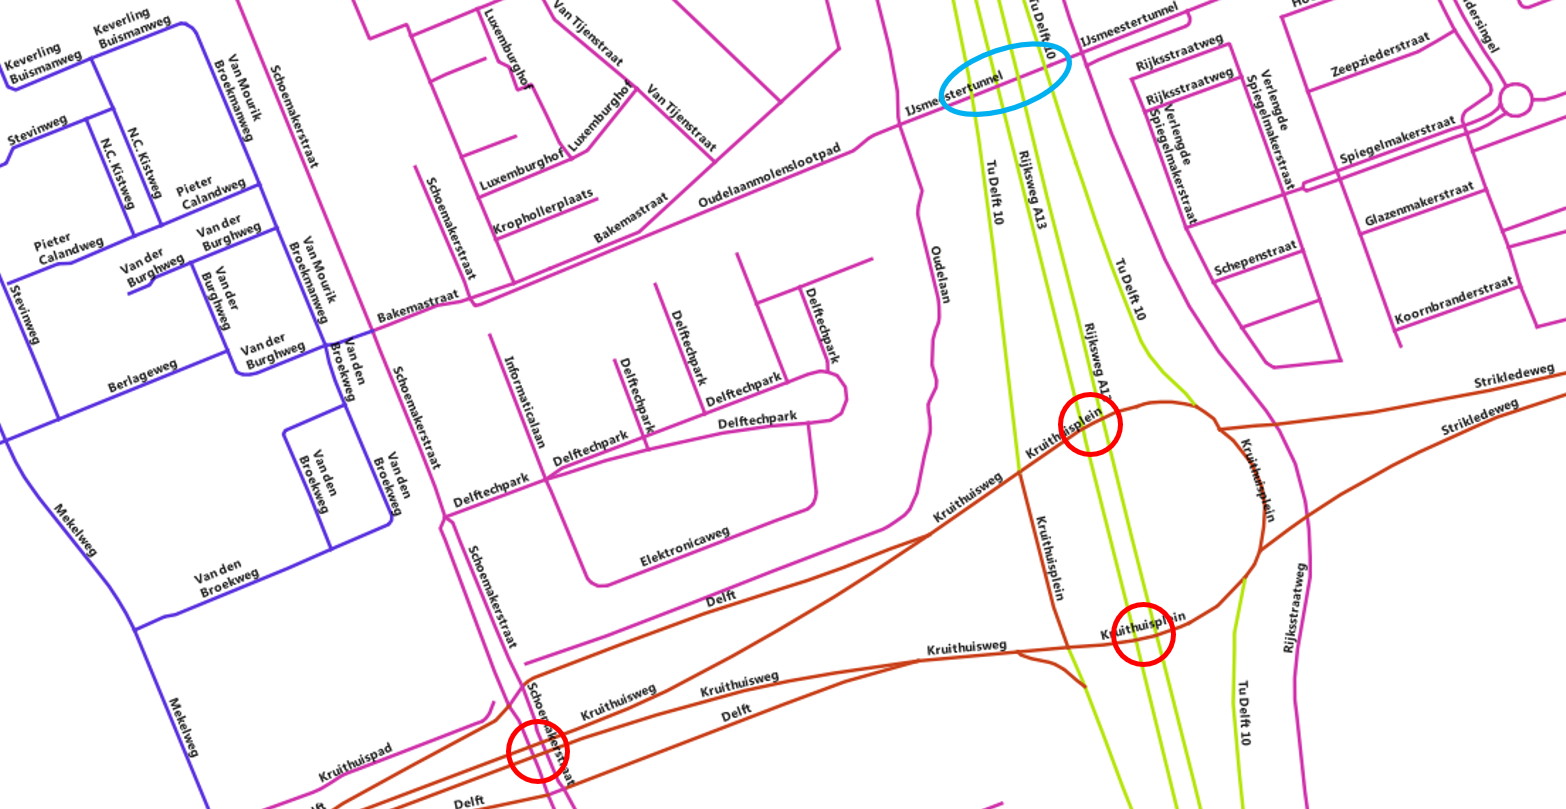
\includegraphics[width=\linewidth]{final_report/figs/nwb_sample_02.png} 
    \caption{An example render of NWB, colour-coded to indicate the owner.}
    \label{fig:nwb}
\end{figure}

NWB (or more specifically, NWB-Wegen, the NWB roads product) is a vector dataset comprised of a semantically enriched set of 2D \textit{MultiLineString} objects released in the \textit{ESRI Shapefile} format. They LineStrings are interconnected in such a way that NWB can be regarded topologically as a graph representation of the Dutch road network. Although NWB contains all named and numbered roads in The Netherlands, we are only interested in roads that are semantically marked as state-owned or province-owned (category R for Rijk and P for Provincie), because the new noise regulation only concerns these types. The NWB product is managed by NDW, but it is owned by RWS (NDW being a division of RWS).

NWB and the road types it contains are illustrated in Figure \ref{fig:nwb}. Yellow is used for R-roads (state-managed roads), red denotes P-roads (province-managed roads) and magenta means G-roads (municipality-managed roads). W-roads (RWS-managed roads) are not shown in this figure. Blue roads (T-roads) are roads which do not fall into the above 4 categories, in this case they are managed by the TU Delft. This render also contains examples of challenging 3D relationships. Where the P-road Kruithuisweg/Kruithuisplein crosses the G-road Schoemakerstraat and the R-road A13, no intersection occurs in 2D because the roads cross over one another in 3D. These locations are indicated in the figure by red circles. Furthermore, where the bike path IJsmeestertunnel (a G-road in NWB) crosses the A13, a series of 3 short tunnels are located in reality. This is indicated in the figure by a blue oval. Although not all these road types are relevant to this project, the 3D relationships represented by these examples still are.

In addition to representing the topology of the road network, the NWB lines are georeferenced with mediocre accuracy to also represent its approximate spatial layout. The quality description includes only a single figure, which is 5 m accuracy at 95\% confidence, i.e. two standard deviations from the mean. It is not described in any detail, how the accuracy is evaluated for each road, for instance whether it is based on the accuracy of the vertex locations of the road, an arbitrary sampling along their length, and how exactly these are aggregated into the error figure. Furthermore, we do not know whether the reference for the accuracy assessment was empirical (surveyed control points) or whether it is purely theoretical and is based on the sources and the methods involved in creating and updating the dataset.

Adding to the uncertainty is the fact that both the topological and the geographical information content of NWB is assembled from a wide range of providers ranging from large national providers such as RWS and Kadaster, to local providers such as specific road authorities and civil engineering agencies. No clear indication is given in the documentation about the sources used for the compilation of specific NWB road types or the estimation of their accuracies, but it is mentioned that they are not the same (\cite{nwb_docs}).

In interpreting the 5 m accuracy, it is important to note that the NWB lines represent road centrelines, but not of the whole paved surface. The centrelines in NWB approximate the centre of the traffic-occupied parts the roads, excluding hard shoulders and other paved surfaces connected to the road. It is also important, that NWB often does not contain vertices for more than 200 m based on my inspection (where roads are relatively straight), and even in sharp bends for up to 20-30 m at a time. Especially in bends, this circumstance, combined with the official error figure, means that NWB often leaves the traffic occupied road surfaces, and sometimes even the paved areas. I confirmed this problem by comparing NWB with DTB, AHN3.

One such comparison is shown in Figure \ref{fig:ahnnwb}. AHN3's ground points are coloured blue in this figure, and NWB centrelines are shown in white. As they have no elevation, they appear below AHN3 points and are consequently masked out partially by them. I shifted them to match AHN3's mean elevation locally, to make them better comparable. Comparisons such as these reveal that NWB gets close to the edges of the paved surfaces quite often, and sometimes even leaves their surface. In sharp bends, this is made worse by the angularity introduced by the coarse lengthwise discretisation of NWB, for instance in the location pointed out by the green arrow. In later stages of the project, I made further comparisons with the BGT and with orthoimagery (Luchtfoto 2020 from Kadaster), discussed in Section \ref{sub:completeness} and with an example shown in \ref{fig:bgtcomparison}. These comparisons further confirmed the issues.

Although the above nominal accuracy and its description are certainly not good enough for compliance with the new noise regulations, the 3D conversion of NWB is not concerned with improving it – in fact, it is a requirement of the project not to displace NWB horizontally. Hence, we may say that the intended outcome of the 3D conversion is to devise a method that can produce accurate elevations for NWB \textit{assuming} that its accuracy complies with the requirements set by the new noise regulations - 20 centimetres at 95\% confidence. To achieve this compliance in practice, lateral refinement is being carried out in a separate project by matching NWB roads with their counterparts in other, more accurate datasets. Specifically, DTB is being used for this purpose, as well as another open data dataset called Basisregistratie Grootschalige Topografie (BGT). As these datasets are already theoretically compliant with the accuracy requirements, correcting NWB geometries based on them will foreseeably solve the lateral accuracy problems of NWB. However, at the time of writing of this report, the BGT-based correction has only been released for municipality-owned roads (category G for Gemeente - not relevant to us), while the DTB-based corrections for motorways are still being finalised. Consequently both the commercial and the scientific 3D-NWB project still rely on NWB data that lacks this correction (\cite{nwb_gecorrigeerd}).

Regardless of improving NWB’s lateral accuracy not being within the scope of this project, it is important to be aware of it, because of its implications when overlaying NWB with AHN3 and DTB in the processing part of this research. The problems caused by it and the necessary workarounds are discussed in-depth in the relevant sections of the next chapters.

The NWB product is updated every month with particular attention to always including new roads, removing outdated (demolished or permanently closed) roads and updating refurbished roads as necessary. This frequency means that NWB is always up-to-date with changes to the road network, at least to the extent where navigation (in e.g. Google Maps, which uses NDW) can take place without any disruptions. However, this does not mean that NWB has a temporal resolution of one month; for that to be true, all roads would need to be re-measured every month. The monthly releases merely mean that effort is concentrated into releasing known changes to the road network frequently. Since no physical phenomena exists that would move the roads laterally (without human intervention) by a significant distance, this does not cause issues in practice.

\begin{figure}
    \centering
    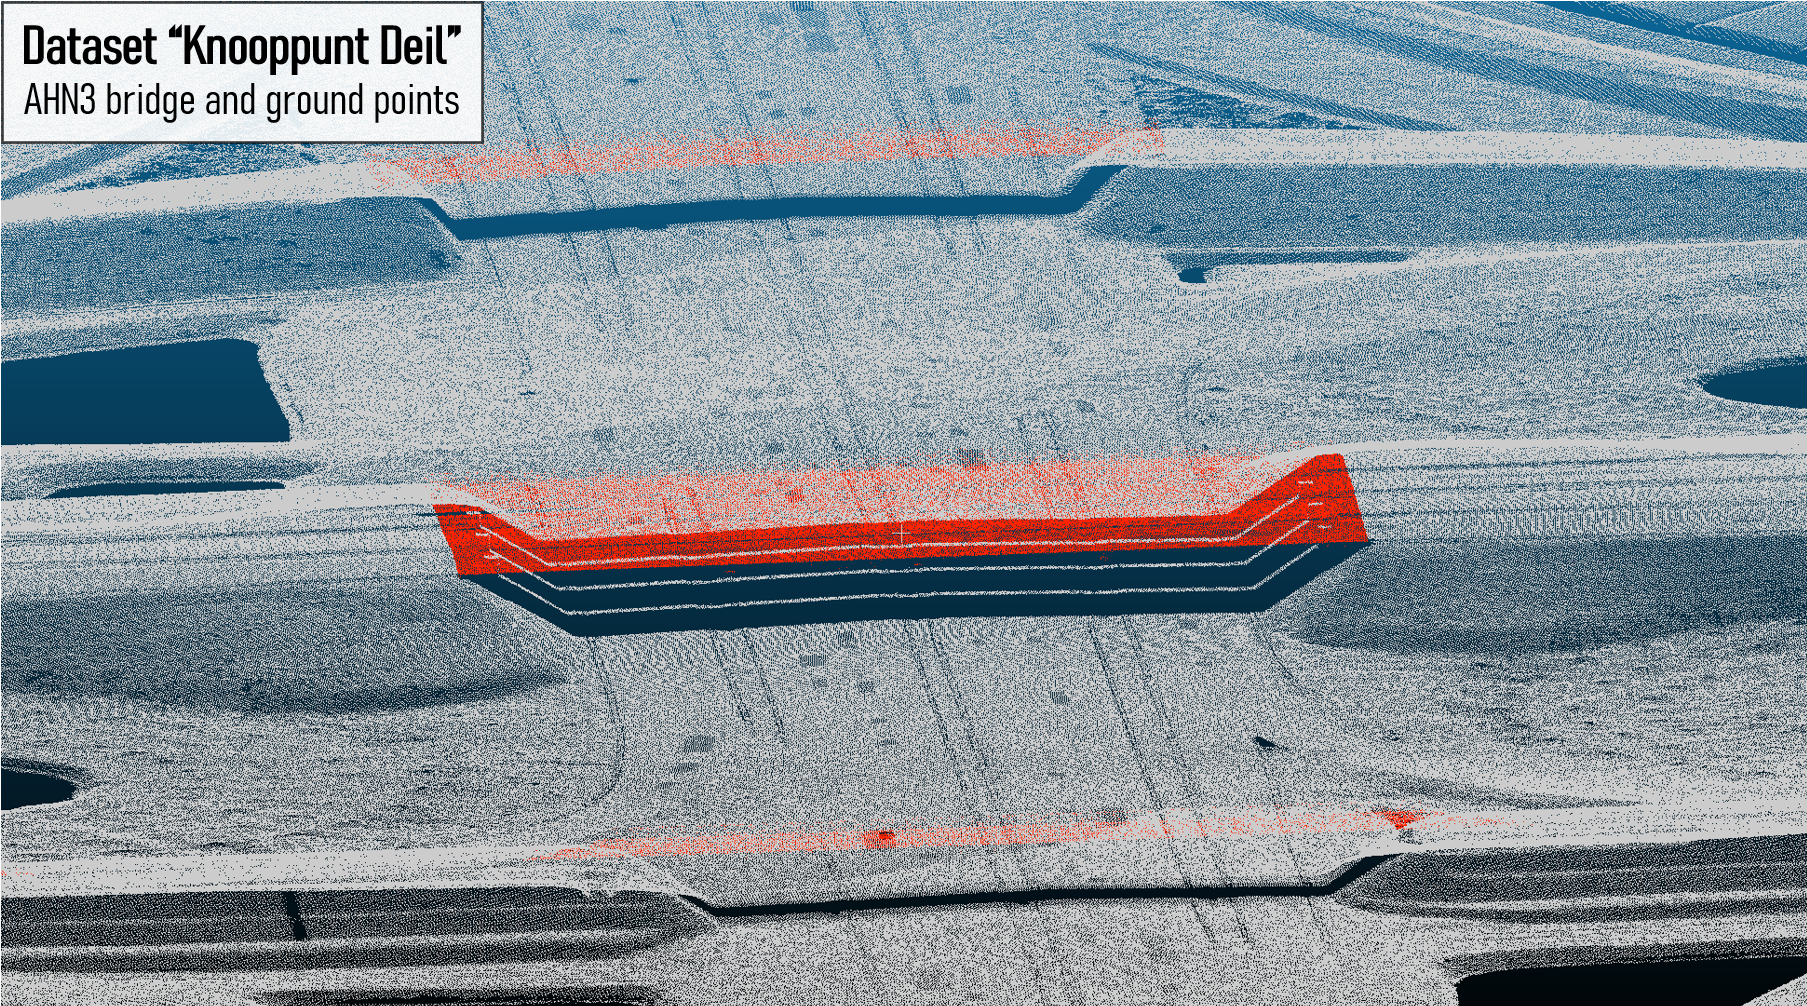
\includegraphics[width=\linewidth]{final_report/figs/ahn_sample_01.png} 
    \caption{Example render of AHN3 at Knoppunt Deil, SW of Geldermalsen, showing ground points and bridges.}
    \label{fig:ahnbridges}
\end{figure}

\subsection{Actueel Hoogtebestand Nederland – AHN}
\label{sub:ahn}

AHN are airborne Lidar (ALS) survey datasets available as open geospatial data in The Netherlands. The surveys are commissioned every few years with AHN (the first version) to AHN3 already complete (1996 to 2019), and the first AHN4 tiles nearing release. At this stage of the project, we are interested only in AHN3, as it is te most recent iteration of this product. The AHN product is owned and managed by RWS.

The dataset has a combined systematic and stochastic elevation error of 15 centimetres at two standard deviations (i.e. 95 \% confidence), and 6 to 10 points per square metre point density on average, corresponding to a 0.32 to 0.41 metre posting distance. The lateral error is 18 centimetres at two standard deviations (\cite{ahn_kwaliteit}). Comparing these to the descriptors of Lidar datasets used in the research examined as part of our literature review (see the Relevant work section), we may assert that AHN3 can be considered accurate, and to have excellent point density. It is especially accurate and dense relative to the older Lidar datasets that are mentioned in these papers, including the first iteration of AHN.

The AHN3 point cloud has been classified semi-automatically with similarly excellent accuracy and is released with the classification included. This means that for most purposes, the point cloud needs not be ground filtered by users, and that extracting certain features is made far easier. Of the various classes available, we are interested in class 2 the most, which corresponds to ground points, and class 26 which contains, among other things, bridge structures and the roads that are found on them.

Ground points are primarily interesting to us because they contain the points reflected from land-based roads. This includes roads that were constructed directly on the terrain, as well as roads constructed on altered terrain, such as elevated ground or open trenches. It also contains the points that represent the terrain in the vicinity of the roads. Elevated roads and bridges are not considered ground points and are generally represented by gaps in class 2, which can, in most cases, be filled by using data from class 26, as shown in Figure \ref{fig:ahnbridges}. The white colour corresponds to ground points (class 2), red corresponds to bridges (class 26). All other classes were removed. The shapes of motorway lanes and ramps, as well as bridges are clearly defined. Road constructed on elevated ground is reliably classified as ground, bridges are cleanly split off by the classification. Even under thin bridges, data becomes gradually sparser at the border and becomes extinct directly below the bridge. This render also makes it clear that wherever vehicles were encountered on ground-based roads, the sampling is worse locally. It does not \textit{generally} go entirely extinct however, as most locations have been scanned multiple times. Data gaps are only observed where slow or stationary vehicles wer encountered.

Class 26 also contains other types of objects, for instance large motorway signs arching over road surfaces, as well as the civil engineering structures of elevated roads and bridges (in addition to the road surfaces on them). Reflections from vehicles transgressing bridges are also present in this class. Figure \ref{fig:ahnsigns} shows a render from the same location as \ref{fig:ahnbridges}. The full-width motorway signs are clearly visible above the motorway lanes, coloured red because they originate from class 26. It also shows that the presence of water results in holes (the dark, linear features running parallel with the motorway in this render) in the ground-only point cloud. In this render, it is also visible that in my testing datasets, all points falling outside a 150-metre buffer zone around the NWB centrelines were removed (see more information on this in Section \ref{sub:testingdata})

\begin{figure}
    \centering
    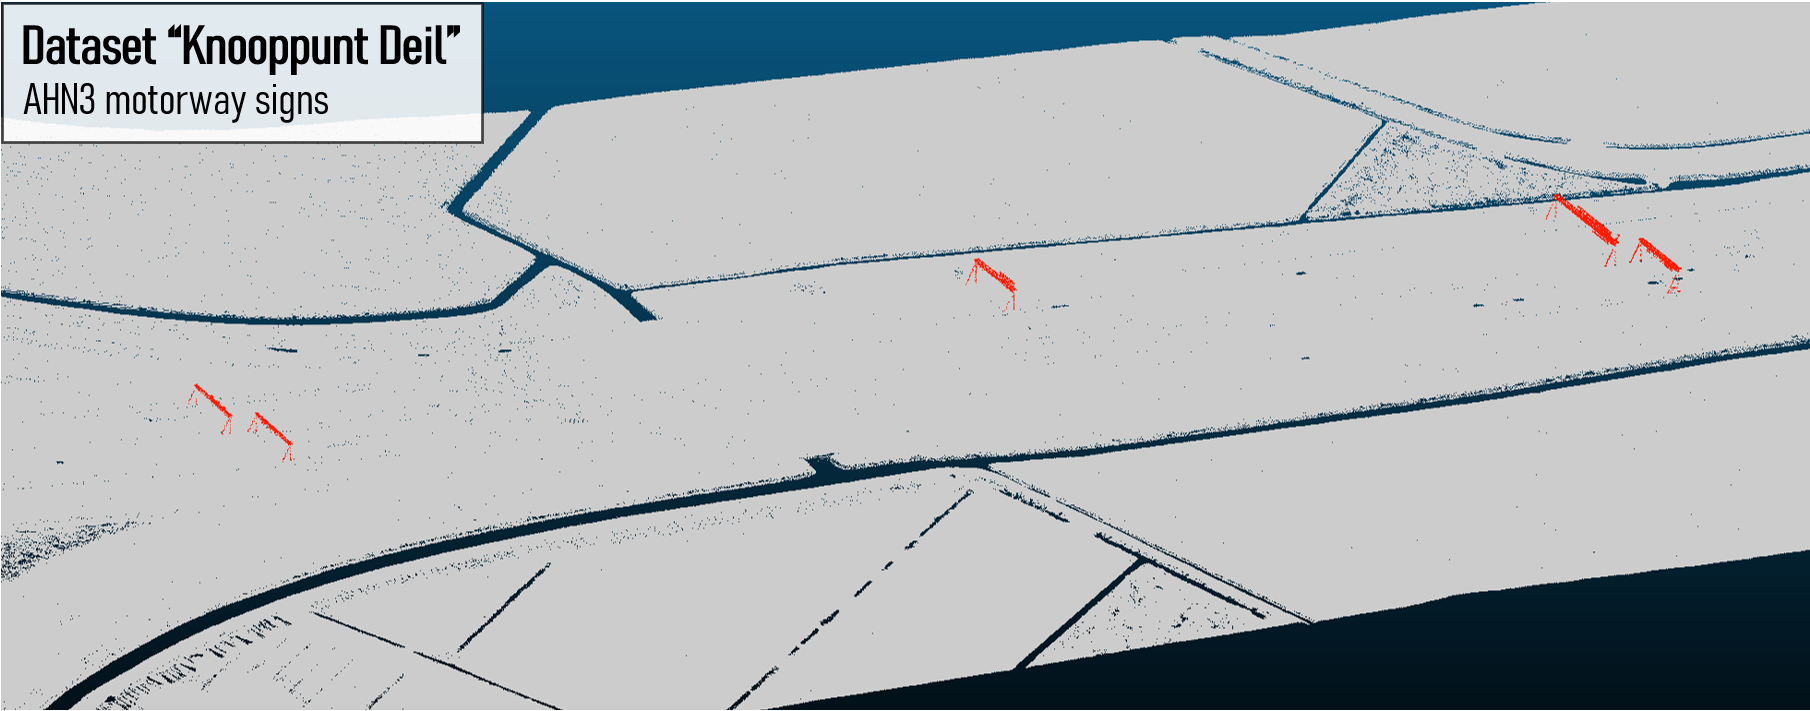
\includegraphics[width=\linewidth]{final_report/figs/ahn_sample_02.png} 
    \caption{Example render of AHN3 at Knoppunt Deil, SW of Geldermalsen, showing ground points and motorway signs.}
    \label{fig:ahnsigns}
\end{figure}

\begin{figure}
    \centering
    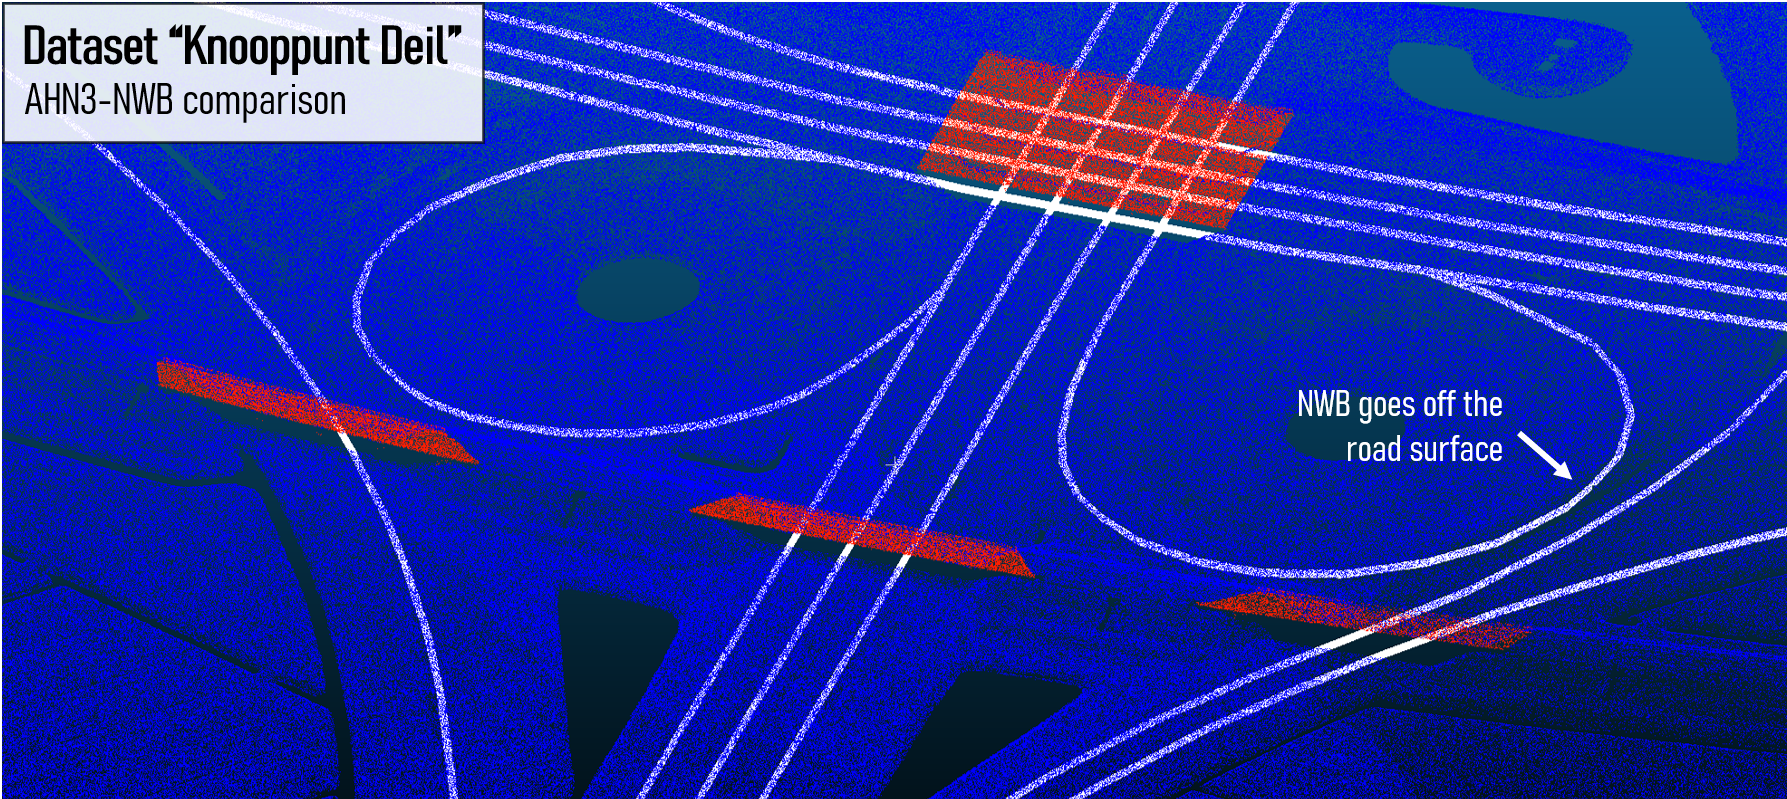
\includegraphics[width=\linewidth]{final_report/figs/ahn_sample_04_a.png} 
    \caption{Render comparing AHN3 with the relevant 2D NWB centrelines.}
    \label{fig:ahnnwb}
\end{figure}

AHN3 is released in the form of a point cloud, as well as DSM and DTM rasters. Both were produced using basic radial IDW interpolation with a fixed parametrisation. The DTM was generated by including only points from class 2 in the interpolation step. They are available at 0.5-metre and 5-metre resolutions, with the 0.5-metre resolution being relevant to this project in terms of the target accuracy. For context, this raster converts (on average) 1.5 to 2.5 points into a single raster cell based on AHN3's nominal sampling density. The commercial implementation uses these rasters, as explained in Section \ref{sub:commercialproduct}.

The Lidar tiles are released in the binary LAZ format (compressed LAS, or LASzip), and are generally several gigabytes in size. As each tile only covers an approximate area of 32 square kilometres and the LAZ compression ratio for this dataset is 0.1 on average, scaling considerations are relevant to this project if the implementation is to be capable of fully converting NWB to 3D using the raw point clouds rather than the rasters.

\begin{figure}[h!]
    \centering
    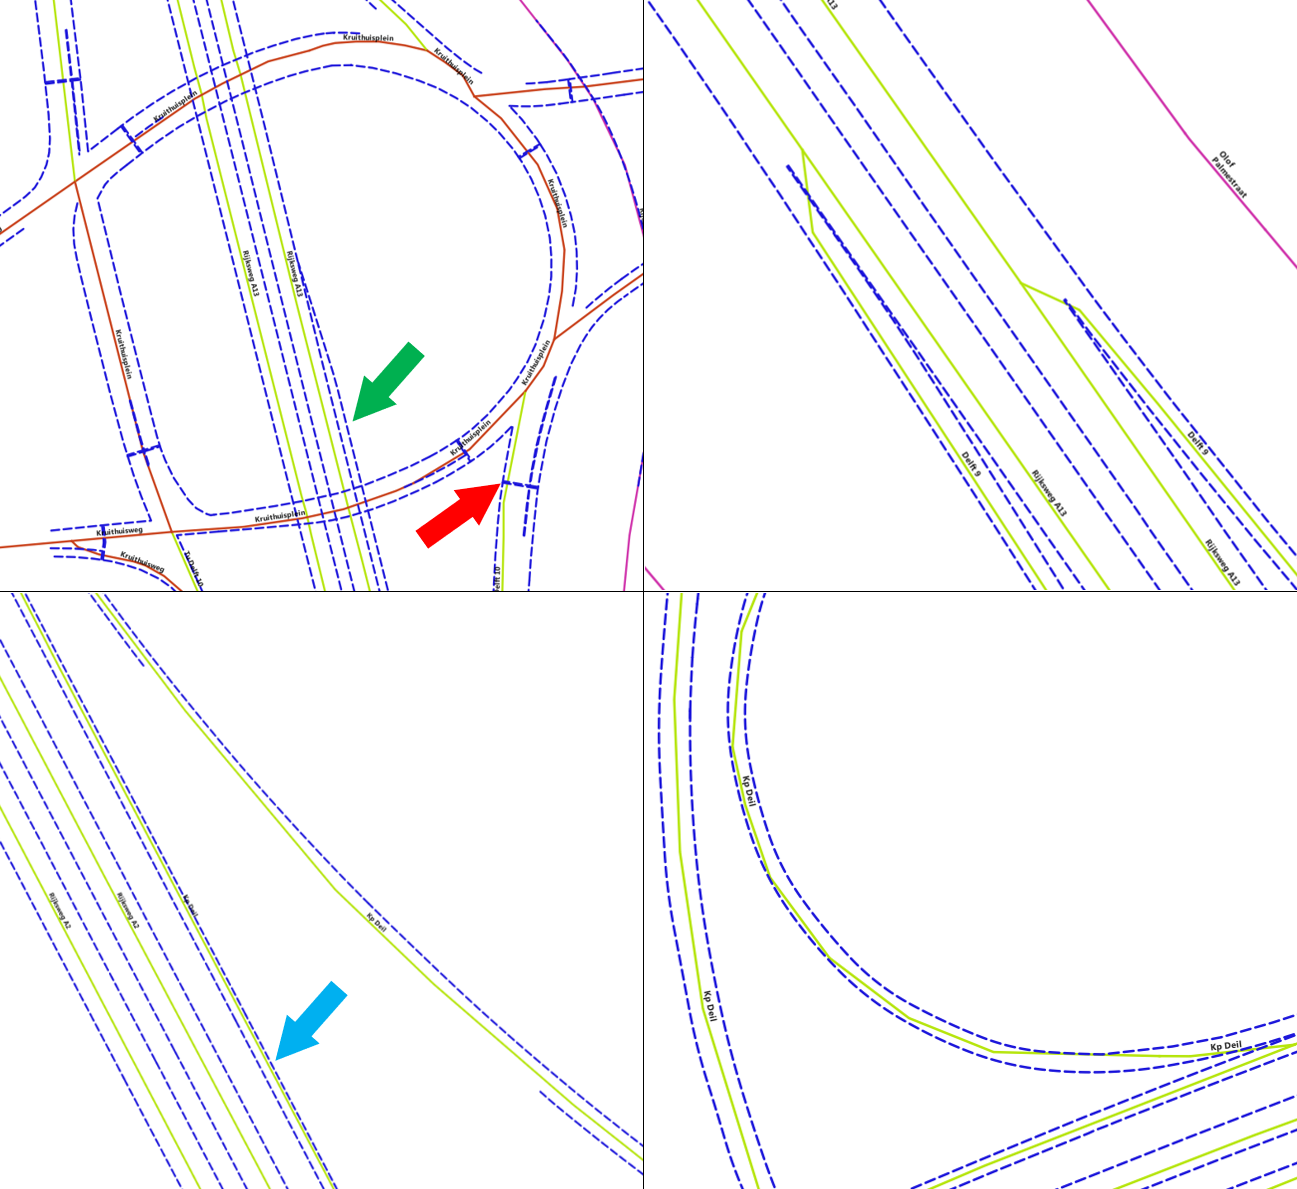
\includegraphics[width=0.95\linewidth]{final_report/figs/dtb_sample_07.png} 
    \caption{Renders of DTB \textit{verflijnen} overlain with NWB centrelines, illustrating "compatibility issues" and individual DTB issues.}
    \label{fig:dtbnwb}
\end{figure}

\subsection{Digitaal Topografisch Bestand – DTB}
\label{sub:dtb}

\begin{figure}[h!]
    \centering
    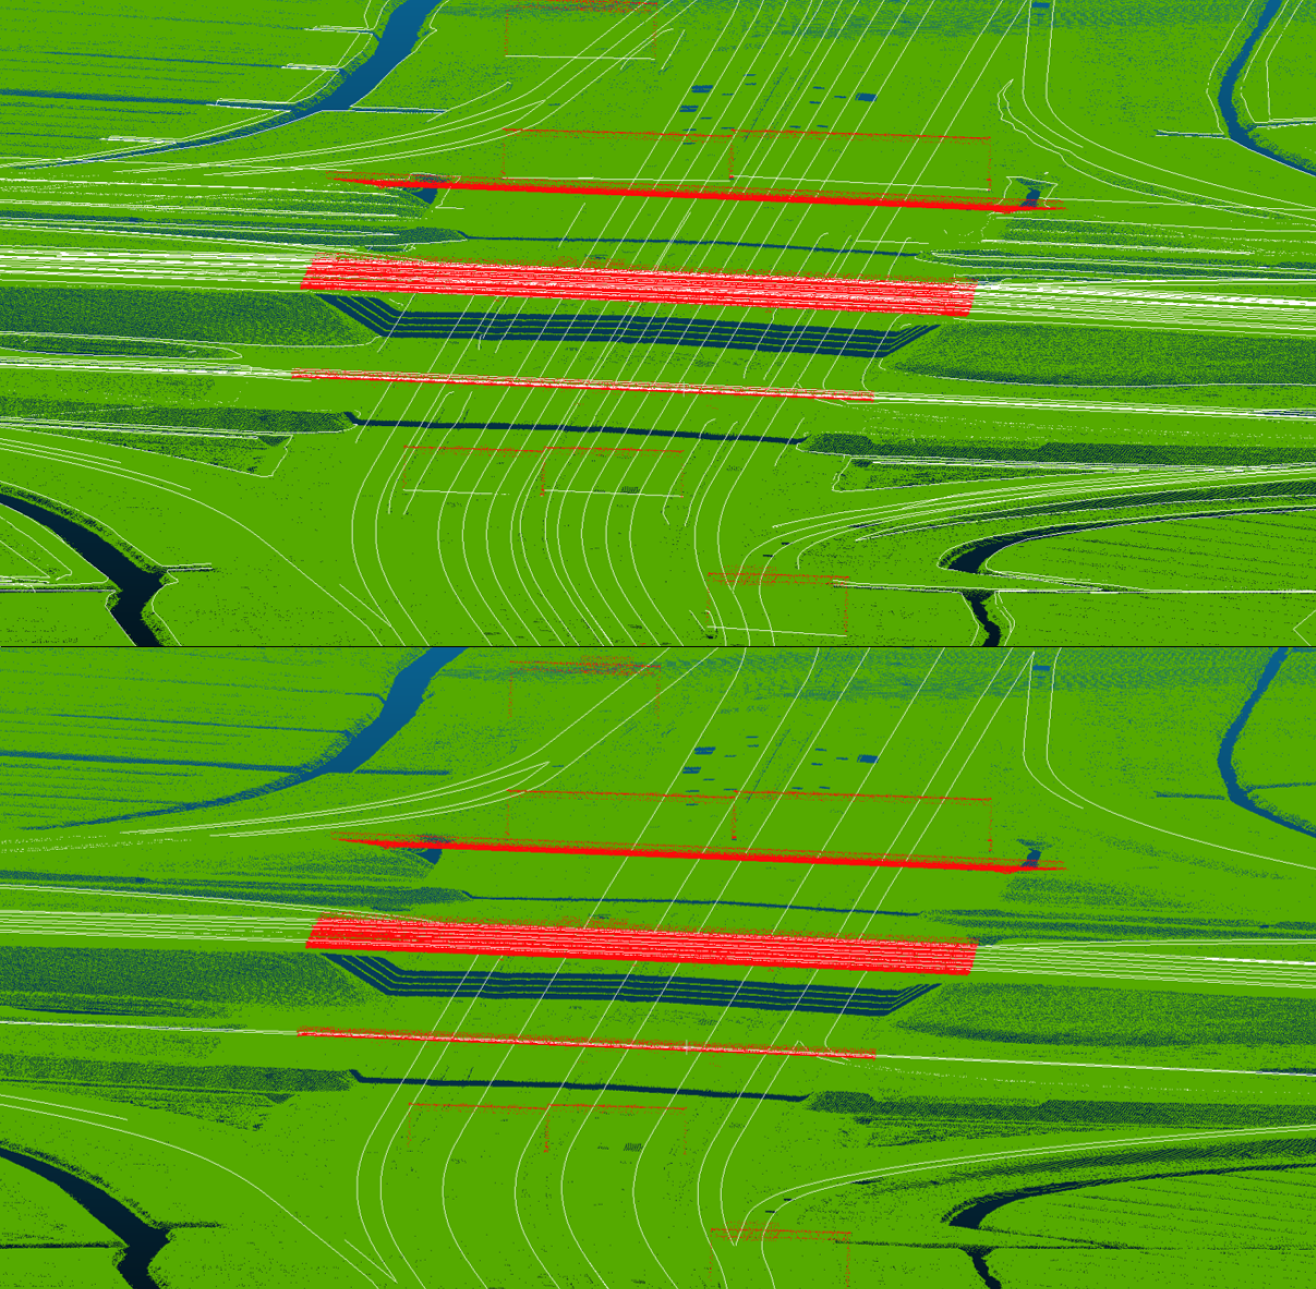
\includegraphics[width=0.95\linewidth]{final_report/figs/ahn_sample_10.png} 
    \caption{Renders of DTB line features overlain with AHN3 in 3D.}
    \label{fig:dtbahn}
\end{figure}

Like NWB, DTB (or more specifically, DTB-Droog, the DTB product relevant to roads) is a Dutch open data geospatial dataset in the \textit{ESRI Shapefile} format. For the purposes of this project, we only need only those DTB line features, which correspond to street surface markings, hence we can also regard this as a dataset comprised exclusively of \textit{MultiLineString} objects, making it identical to NWB in its data structure apart from being a 3D dataset. DTB is also managed by RWS and it is concerned only with state-owned roads and roads on state-leased land, which translate almost exclusively to NWB R-roads, that is, motorways. DTB is, hence, not a reliable source of information about provincial roads elevations (NWB P-roads), our other road type of interest.

There are various types of DTB road markings that are of interest to us, the main one being a category called \textit{verflijnen}. These DTB lines represent the painted lines marking the outermost edges of the area open to traffic. This is a lucky correspondence with NWB, as it too, contains the centrelines of the areas of roads that are open to traffic. The other two types I found to be reliably represent road surface elevations are the categories \textit{verfstippellijn} and \textit{blokmarkering}, which are lane separation lines and block marks respectively. The category \textit{lijnverlichting} also appeared to be interesting at first, as it corresponds to road surface lighting features (not street lighting). However, I found it to not be reliably located on road surfaces in practice, hence I excluded it from further consideration.

Figure \ref{fig:dtbnwb} shows a visual comparison with NWB, illustrating various types of significant issues that primarily stem from NWB's crude georeferencing. NWB symbology is identical to that which I used in \ref{fig:nwb}, and blue dashed lines are the DTB lines. Only \textit{verflijnen} are present in DTB in these locations. The image in the top left shows that in practice DTB contains many road markings, rather than just one on either side of NWB. The illustration in the top right shows that NWB motorway ramps often merge with the motorway lanes at unrealistic angles, causing NWB to intersect the DTB edge markings at these locations. The image in the bottom left illustrates that while in some places there are many DTB road edges, in other places they are incomplete or missing entirely. Furthermore, NWB centrelines may also get very close to DTB edges outside of sharp bends and motorway ramps, as indicated by the blue arrow. In the bottom right, the figure shows that NWB discretisation and inaccuracy leads to angular angular lines in sharp bends. NWB often gets close to, or even intersects DTB in such places.

Like NWB (but unlike AHN3), DTB’s production pipeline also concerns several organisations performing various types of sensing, which are then semi-automatically assembled into the complete DTB product. While many DTB features are photogrammetry-derived, road surface markings are mainly from accurate land-based manual surveys or extracted from car-mounted Lidar (MLS) data (\cite{oudeElberink_vosselman_2012}). The documentation of DTB consists of its formal specifications (\cite{dtb_docs}) and a handbook (\cite{dtb_handbook}). The former contains the accuracy-related details, reporting 10 cm vertical and 5 cm horizontal standard deviations, or 20 cm and 10 cm at 95\% confidence to make it comparable with the reported accuracy of NWB and AHN3.

Theoretically, DTB is not only accurate, it also has a good temporal resolution. It is updated multiple times a year, specifically to always be up-to-date in terms of newly constructed roads and refurbished roads - just like NWB. This update frequency is comparable to that of NWB, which is part of the reason why it forms part of the commercial solution. The other part of the reason is, that it theoretically always contains data for occluded roads, even in tunnels. This means that the combined information content of DTB and AHN3 theoretically amount to having complete coverage of the Dutch road network. Because of the ease with which elevations can be extracted from DTB to be used in the 3D conversion of NWB (especially considering the crudeness of NWB's georeferencing) prompted NDW to consider DTB as its \textit{primary} dataset, wherever it is available.

In practice, I found evidence to support that the above decision is fundamentally flawed, already during the input assessment stage of my project. There are places where DTB lives up to the above \textit{theoretical} standards, but this is not the case in most of the areas I examined. Even in terms of motorways, DTB is often incomplete to the extent that it lacks coverage over tens of kilometers. Even where it exists, its coverage may be patchy, especially in sharp bends. An example is shown in Figure \ref{fig:dtbnwb}. Commonly it only contains a single line rather than the theoretical minimum of three (two edge markings and one separation line). The separation line is the one I observed to be missing the most frequently.

Furthermore, already by considering the update methodology of the dataset, one may remark that some of the elevation measurements in it must be very outdated. Indeed, most of them are almost as old as the roads themselves, meaning that they were taken more than 20 years ago. This is where it comes into play that the update methodology of NWB and DTB does not really represent a high temporal resolution. In the absence of a physical phenomenon causing significant lateral ground motion, this does not cause problems with NWB, but there \textit{is} one that may move roads up or down: subsidence. Although the surface load due the weight of the road and passing vehicles may play a role, subsidence is primarily caused by natural, geological processes. In some parts of The Nethelands, groundwater and natural gas extraction may also play a role. Although this work does not specifically study the correlation between subsidence and problems with DTB, there is little else with which the 0.5 to 1 m differences between AHN3 and DTB could be explained. The AHN3 measurements are at least 15 years more recent than the oldest ones in DTB, which is where the biggest differences can be observed in elevation, as one would expect from subsidence.

Interestingly, the opposite can also be observed, although less commonly, and in a highly localised manner. In some places, DTB is above the road surface measurements of AHN3 by a significant margin, often by more than 0.5 m. While subsidence cannot be used to explain these disagreements, there is evidence to support that the elevations in AHN3 are indeed correct and the ground has shifted upwards noticeably. The latest subsidence survey of The Netherlands reported positive changes in addition to the decreasing elevations that are associated with subsidence. I primarily observed DTB to be below AHN3 where this map indicates negative elevation changes, and above in regions where no changes or slightly positive changes were observed in the subsidence study, verifying my hypothesis.

Figure \ref{fig:dtbahn} shows renders of DTB overlain on AHN3 with all DTB features shown (above), and with only \textit{verflijnen} shown (below). Ground points are shown in green. The top render illustrates that other features, such as roadside slopes, canals, ditches, safety rails are represented in DTB. Full-width motorway signs are also occasionally represented (either by lines on the road, or on the structure itself). The bottom render shows that locally, the edge markings are in good agreement with AHN3 visually, and are only occasionally incomplete. This location has the best vertical correspondence with AHN3, and also the best completeness, of all the areas I examined. For illustrations of the \textit{disagreements} between DTB and AHN3, please refer to Figure \ref{fig:lidarsegmentation1} and the associated discussion in Chapter \ref{chap:r}.

\section{Methods of existing implementations}
\label{sec:methodsexisting}

\subsection{NDW prototype}
\label{sub:ndwprototype}

NDW themselves produced a prototype implementation, which can achieve a 3D enrichment of NWB with only a few gaps in the produced elevation profiles. Although their workflow does not have a formal documentation, I have been given a verbal description of it, as well as the output. Based on my understanding of these, their primary technique involved snapping close-by AHN3 Lidar points to the line geometries of NWB. Notable problems with the implementation included non-road points being snapped to centrelines, causing road centrelines to be given overestimated elevations, in turn resulting in abrupt spikes in the elevation profiles.

Furthermore, no close-by points could be found for underground roads (i.e. tunnels), and strongly occluded parts of roads. For small gaps, this was resolved partially by writing an algorithm to interpolate linearly inside NWB, using the closest vertices where snapping was successful. For larger gaps, an attempt was made to resolve issues by including information from external sources semi-automatically. Neither issue could be fully resolved via these approaches, hence the results of this project were only used by NDW to gain a better understanding of the problem and the expected challanges. For the development of a reliable digital toolbox they subsequently commissioned a commercial implementation from RHDHV.

\subsection{RHDHV's commercial implementation}
\label{sub:commercialproduct}

RHDHV developed their implementation in parallel with the planning of the present scientific research. During this time, I attended NDW-RHDHV meetings, discussed the commercial system design and implementation details directly with RHDHV personnel, and was granted access to the codebase of the project. Understanding their implementation was crucial for the planning and realisation of my research, as it was among my goals to estimate the effectiveness of the commercial implementation's methods, as well as assess the quality estimate the accuracy of the their final results. In addition, creating my system design while learning about the known and suspected shortcomings of their methods allowed me specifically focus on areas where a different, less pragmatic approach could yield better results.

\subsubsection{Overview of system design}

First, where NWB vertices are too sparse, vertex densification takes place; i.e. additional vertices are created inside NWB line segments until all vertices are found less then a certain threshold distance from their neighbours. From then onwards, \textit{different} workflows are initiated for R-roads and P-roads.

For P-roads (where DTB data does not generally exist), the workflow is conceptually similar to the one in the prototype, with the notable difference of using AHN3 DTM rasters rather than the point cloud. Because AHN3 DTM rasters are badly affected by both large holes and small groups of missing pixels (due to the fixed-parameter IDW interpolation that was used to generate them), RHDHV could only make use of them by filling in the gaps of the raster using linear interpolation in a 3D TIN created from extruded raster pixel centres. They then simply interpolated elevations for NWB from the raster using bilinear interpolation. Intermediate results of this procedure are shown on the right in \ref{fig:rhdhv}. It shows a raster being overlain with NWB to yield elevation values. The raster still contains the holes that AHN3 rasters contain by default; these are filled in before interpolating elevations for NWB but are shown here for demonstration purposes. Two types of holes generally occur: small-scale ones due to objects such as street furniture, vehicles and vegetation, and large ones that are typically due to large-scale occlusion due to buildings or bridges (as in this case). The test build shown here used AHN2 rasters, but their production implementation uses AHN3.

\begin{figure}
    \centering
    \includegraphics[width=\linewidth]{final_report/figs/rhdhv_combined.png}
    \caption{Illustrations of RHDHV's commercial implementation.}
    \label{fig:rhdhv}
\end{figure}

For R-roads, DTB is available, and the assumption is made that it is more accurate than AHN3 (or at least the stock DTM tiles generated from AHN3), to the extent where it should be the primary source of elevation data. Priority is thus always given to it in the procedure, with AHN-based interpolation used only as a fallback mechanism in case DTB-based height estimation fails for any reason (anomalous elevations computed, or missing DTB geometry).

The goal of the underlying algorithm is to find the closest, roughly parallel DTB line segments at any NWB vertex, and to deduce elevations from them. First, 2D cross-sections are constructed on NWB vertices, with each given the mean azimuth of the two NWB line segments that they are part of, and then rotated 90 degrees. For vertices created during densification, this simply means the rotated azimuth of their parent line segment. DTB lines are then intersected with the cross-sections and for each cross-section, the closest DTB line that satisfies a relative angle condition is picked on both sides of NWB. Elevation is then first linearly interpolated inside the two chosen DTB segments to yield values exactly at their intersections with the cross-section. Lastly, elevation is interpolated linearly along the cross-section itself to yield the final elevation at the location of the NWB vertex.

The angle condition I mentioned above is a threshold-based evaluation concerning the angle between intersected DTB line segments and the cross-sections, and is used to ensure that the chosen DTB segment is indeed roughly parallel to NWB locally. This helps ensure that the algorithm does not accidentally choose a DTB line segment that belongs to a different (underlying or overlying) road surface. The assumption is thus made that the DTB line segments representing surface features of a given road are roughly parallel with the relevant NWB centreline, and lie close to them. Implicitly, this also assumes that even if no other DTB road markings are present, NWB centrelines will still lie between two DTB road \textit{edge} markings, i.e. \textit{verflijnen}.

In practice, backup mechanisms needed to be implemented because these assumptions do not always hold. Primarily, this is because in sharp bends NWB may not be parallel with the relevant DTB lines locally, and because it is frequently not complete enough to be used for the above operations. To bridge these issues, wherever the algorithm only finds a suitable DTB intersection on \textit{one} side of NWB, it is only that side from which the elevation value is deduced. If no suitable intersection can be found whatsoever, the AHN3 raster-based interpolation is used instead (the same workflow that is always used for P-roads).

This procedure is illustrated on the left in \ref{fig:rhdhv}. The cross-sections that are constructed on NWB vertices are shown as black lines. Green circles denote those vertices where the cross section could be properly intersected with DTB lines (blue circles) and thus be given an elevation value. White circles denote where the procedure failed, and AHN raster-based interpolation was necessary. This render illustrates that in sharp bends the assumption that NWB and corresponding DTB lines are parallel does not necessarily hold, because of how coarse and inaccurate NWB's georeferencing is, especially relative to DTB which is very accurate horizontally. The render also illustrates that P-roads are not processed in this way, not even if they have DTB lines next to them (which frequently occurs in the vicinity of motorways).

\subsubsection{Potential limitations}

At the time of finalising this report, the results of the commercial implementation have already been made available to me and the comparison with my own results carried out. However, in this section I discuss the \textit{suspected} limitations of their methods, not the properties of their results. During the project planning, system design and implementation stages, the commercial results were not available to me yet and as a result, the bulk of my work - almost everything apart from Section \ref{sec:r_comparison} - is based on verbal descriptions of their methods and preliminary results.

First and foremost, I suspected that using AHN3 rasters in place of the point cloud would affect the quality of their conversion. Point cloud to raster conversion is, by definition, associated with inherent information loss (less raster cells than point cloud points), and further reduction in accuracy is introduced by the interpolation mechanism itself, that created the rasters. Radial IDW was used to generate AHN3 DTM tiles, which several of the reviewed papers found to be specifically unsuitable for interpolating large-scale areas in which zones of decreased point density or gaps exist – both of which characterise ground-filtered AHN data (e.g. \cite{guo_etal_2010}). In addition, the procedure performs another layer of interpolation to infill gaps, which may further deteriorate accuracy. Furthermore, RHDHV uses bilinear interpolation inside the raster to produce NWB elevations, which is suggested by \cite{shi_etal_2005}, to be less accurate than other common methods such as bicubic.

Furthermore, there is no mechanism built into the software to deal with occlusion in the case of P-roads, and also R-roads where DTB is unavailable. This means that wherever NWB elevations are interpolated in occluded road segments from AHN3 rasters, they will be incorrect. Just like in the NDW prototype, these values will show up as spikes in the elevation profiles, as well as longer bumps where wide features (e.g. bridges) are encountered. Since there is no outlier filtering or smoothing algorithm built into the software either, the severity of this issue is not mitigated in any way.

Based on the input assessment, it is also evident that prioritising DTB wherever it is available may itself be a questionable decision, in view of the fact that the output's accuracy needs to measure up to the noise regulation's expectations, at least theoretically. DTB is accurate horizontally, in fact it is theoretically more accurate than AHN3. However, even if its vertical accuracy was also satisfactory at the time of its acquisition, it no longer is, due to various degrees of vertical ground motion taking place in the country. As elevations in DTB are not updated where no civil engineering changes have taken place in the road network, its road surface markings are often far too outdated to be used with any certainty, especially considering that there is no reason to do so given that AHN3 contains equally accurate, but significantly more recent data.

Lastly, the commercial implementation lacks a formal accuracy assessment. Although this is common with comparable commercial products, in this case the output dataset needs to comply with formal accuracy \textit{requirements}. Without a quantitative or at least qualitative accuracy assessment of some form, there is not enough evidence to support the applicability of the commercial results to the noise modelling applications they are intended for.

Since the accuracy of AHN3 rasters is known and simple bilinear interpolation is used to obtain elevations from them, deriving output accuracy would not be difficult wherever their solution uses AHN3. This excludes interpolating in gap-filled pixels, which would need further considerations. In the case of DTB, the evaluation of accuracy may be equally simple, as the underlying computations all boil down to linear interpolation. However, wherever DTB data is old, any accuracy quantification would be meaningless because DTB itself does not comply with its own formal accuracy, due to vertical land motion.
%!TEX root = thesis_proposal.tex

\chapter{Tools and Datasets}
\label{chap:td}

\emph{[Section to be written]}
%!TEX root = thesis_proposal.tex

\section{Methodology}
\label{sec:m}

This section will first present the methodology employed by NDW to produce the prototype implementation and the one implemented by RHDHV to produce the commercial toolbox. It will then present a detailed overview of my proposed research methodology, separating the processing and the accuracy assessment procedures into two separate workflow descriptions.

NDW themselves produced a non-commercial prototype implementation, which can achieve a 3D enrichment of NWB with only a few gaps in the produced elevation profiles. Although their workflow does not have a formal documentation, I have been given a verbal description of it, as well as the output. Based on my understanding of these, their primary technique involved snapping close-by AHN3 Lidar points to the line geometries of NWB. Notable problems with the implementation included non-road points being snapped to centrelines, causing road centrelines to be extruded to overestimated elevations, in turn resulting in sudden jumps in the elevation profiles. Furthermore, no close-by points could be found for underground roads (i.e. tunnels), and strongly occluded parts of roads. For small gaps, this was resolved partially by writing an algorithm to interpolate linearly inside NWB, using the closest vertices where snapping was successful. For larger gaps, an attempt was made to resolve issues by including information from external sources semi-automatically. Neither one of these issues could be fully resolved via these approaches, hence the results of this project were only used by NDW to gain a better understanding of the problem and the expected challanges. For a reliable, commercial toolbox they subsequently commissioned an implementation from RHDHV.

RHDHV developed their implementation in parallel with the \textit{planning} of the present scientific research. I have attended NDW-RHDHV meetings, discussed the implementation directly with RHDHV, and was granted access to the codebase of the project. Understanding their implementation is crucial for this research, as it aims to both assess the accuracy of the commercial implementation, as well as, in part, base its methodology and implementation on the suspected shortcomings on the commercial implementation. First, where NWB vertices are too sparse, densification takes place and additional temporary vertices are created inside NWB line segments. Then, \textit{different} workflows are initiated for R-roads and P-roads. For P-roads (for which DTB data does not generally exist), the workflow is conceptually similar to the one in the prototype, with the notable difference of using AHN3 DTM rasters rather than the point cloud. Because AHN3 DTM rasters are badly affected by both large holes and small groups of missing pixels (due to the fixed-parameter IDW interpolation that was used to generate them), RHDHV could only make use of them by filling in the gaps of the raster using linear interpolation in a 3D TIN created from the raster pixel centres and their elevations. They overlaid the raster tiles with NWB vertices (including the dense, temporary vertices) and interpolated their elevations using bilinear interpolation inside the raster. For R-roads DTB is available, and the assumption is made by RHDHV that it is more accurate than AHN3 (or at least the stock DTM tiles generated from AHN3), to the extent where it should be the primary source of elevation data. Priority is thus given to it in the procedure, with AHN-based interpolation used only as a fallback mechanism in case DTB-based height estimation fails. The goal of the procedure is to find the DTB line segments that delineate the road edges at any given location in the NWB and deduce elevations from them. First, 2D cross-sections are constructed on NWB vertices, with each given the mean azimuth of the two NWB line segments that they are part of, and also on densified vertices, which receive azimuth values based simply on the azimuth of their parent line segments. DTB lines are then intersected with the cross-sections and for each cross-section, the closest DTB line that satisfies a relative angle condition is picked on both sides. Elevation is then first linearly interpolated inside the two chosen DTB segments to yield values exactly at their intersections with the cross-section. Then, elevation is interpolated linearly along the cross-section itself to yield the final elevation of the NWB vertex or densified temporary vertex. The angle condition is a threshold-based evaluation concerning the angle between intersected DTB lines and cross-sections and is intended to ensure that the chosen DTB segment indeed represents the edge of the current road, rather than some other feature, or the edge of another road. Hence, the assumption is made that the DTB line segments representing road edges are roughly parallel with the relevant NWB centrelines and lie close to them. Implicitly, this also assumes that NWB centrelines will lie between DTB road edges. In practice, none of these assumptions holds in general, hence a range of failsafe mechanisms needed to be implemented. Wherever the algorithm only finds a suitable DTB intersection on one side of NWB, it is only that side from which the elevation value is deduced. If no suitable intersection can be found whatsoever, the AHN3 raster-based interpolation is used instead. At NWB centreline end vertices (where no intersection exists, i.e. dead ends), the previous vertex’s elevation is simply repeated. The described methodology is illustrated in Figure \ref{fig:rhdhv}. It is worth mentioning that the RHDHV implementation deals with all non-standard input data sets (i.e. small-scale engineering models, road management datasets, etc.) by first converting them to rasters with the same specifications as AHN3 DTM tiles and mosaicking them into an output raster based on a priority list, before filling in any remaining gaps and interpolating bilinearly.

\begin{figure}[h]
    \centering
    \includegraphics[width=\linewidth]{p2/figs/rhdhv_combined.png}
    \caption{Illustrations of RHDHV's commercial implementation. \textbf{Left:} The cross-sections that are constructed on NWB vertices are shown as black lines. Green circles denote those vertices where the cross section could be properly intersected with DTB \textit{verflijnen} (blue circles) and thus be given an elevation value. White circles denote where the procedure failed, and AHN raster-based interpolation was necessary. This render illustrates that in sharp bends (where the cross-section might not intersect DTB orthogonally) and close to intersections, this workflow often fails, and that P-roads are not processed in this way (they have DTB edges in this particular location only because they are close to R-roads). \textbf{Right:} AHN-based interpolation is used for P-roads, and as a fallback mechanism where DTB-based interpolation fails. The rasters are overlain with NWB to yield elevation values, and as the DSM rasters contain holes, they are patched in by pre-interpolating them before this step. In this illustration, the holes are left in to show that two types of holes generally occur: small-scale ones due to objects such as street furniture, vehicles and vegetation, and large ones that are typically due to occlusion from overlapping buildings or bridges (as in this case). The test build shown here uses AHN2 rasters.}
    \label{fig:rhdhv}
\end{figure}

There are various sources of issues that I this methodology suggests, from a scientific point of view. For instance, point cloud to raster conversion is, by definition, associated with inherent information loss (less raster cells than pixels), and further reduction in accuracy is introduced by the interpolation mechanism itself. Radial IDW was used to generate AHN3 DTM tiles, which several of the reviewed papers found to be specifically unsuitable for interpolating large-scale areas in which zones of decreased point density or gaps exist – both of which characterise ground-filtered AHN data (e.g. \cite{guo_etal_2010}). In addition, the procedure performs another layer of interpolation to infill gaps, which may further affect accuracy negatively. It is also worth mentioning that RHDHV uses bilinear interpolation inside the raster to produce NWB elevations, which is suggested by \cite{shi_etal_2005}, to be less accurate than other common methods such as bicubic. In terms of their strong prioritising of DTB for R-roads, I should remark that DTB is also a secondary source of information (it is based on procedurally combining various types of sensing into vector features), and in contrast with AHN3, neither its overall nor its local accuracy are reported in its documentation or known from elsewhere. While it no doubt contains valuable information that may benefit the overall procedure, relying on it as the sole source of elevation data may not be an approach that can guarantee the levels of accuracy needed for SWUNG2 compliance.

My proposed approach is the result of a combined understanding of concepts in related work, my own knowledge and experience relating to geomatics concepts and methods, as well as inspiration from the commercial implementation of RHDHV. The proposed workflow was built with the research questions in mind. The below summary is only a top-level description, as I expect the detailed specifications to change.

\begin{enumerate}
    \item Pre-processing
    \begin{enumerate}
        \item Keep only NWB R-roads and P-roads. Identify \textit{non-branching road segments}, henceforth referred to as \textit{NBRSs}. To identify them, first look for interconnected networks of MultiLineString objects sharing the same street name, then split off branches at intersections, always doing so in the order of decreasing angle (to ensure that a straight continuation of roads is natively preferred). Perform vertex densification for NBRS edges longer than a set distance.
        \item Keep only AHN3 points within a set distance from NWB lines. Keep classes 2 and 26 only.
        \item Keep only DTB “verflijnen”.
    \end{enumerate}
    \item Point cloud partitioning
    \begin{enumerate}
        \item For each NBRS from the previous stage, fit planes to the neighbourhood of edges and fetch points that are close to them. When selecting a final plane from candidate planes, perform a similarity check between the parameters of neighbouring planes, so that the resulting succession of planes are not oriented unrealistically with respect to each other. Determine the exact procedure and parametrisation in a way that it is not too complex computationally, but still captures most Lidar points relevant to the given NBRS (i.e. do not use conservative thresholds at this stage).
        \item Merge the sub-clouds of edges into a single sub-cloud for the NBRS and save to disk with an identifier linking it to the NBRS itself.
    \end{enumerate}
    \item Road edge identification
    \item[] To be performed on each generated NBRS (and linked sub-cloud of Lidar points).
        \begin{enumerate}
            \item Construct cross-sections on NBRS vertices (including densified vertices) and snap close-by AHN3 points to them at a pre-set sampling distance along each of them.
            \begin{enumerate}
                \item Find the dominant line parametrisations of their elevation profiles and discard non-conformant points.
                \item Disregard points separated by gaps (created by the previous step) from the main group of points representing the fitted line (close to NWB), and points outside a maximum allowed road width. The outermost points in the detected series represent the approximate local position of the road edge on each side.
                \item Disregard cross-sections where steps i. or ii. indicate that locally, NWB does not lie on the road surface as suggested by AHN3 (for instance, because the cross-section regression line does not cross the centreline in 2D).
                \item Derive mean elevations for each cross-section from the remaining points.
            \end{enumerate}
            \item The series of mean elevations (one per cross-section) is itself a 1D elevation profile. Perform outlier detection by sliding a kernel along this profile. Discard cross-sections where this operation indicated that the fitted line is significantly above the road surface. This will help eliminate cross sections corrupted by local groupings of non-road points (such as class-26 motorway signs).
            \item Assemble approximate global road edges from the two outermost Lidar points (on each side of NWB) of each cross-section kept after the pervious step.
            \item Use the left and right road edge estimates from the previous step as initial approximations in an active contour optimisation step. The constraints (energy terms): realistic horizontal distance from NWB for Dutch roads, and/or realistic distance from its own initial edge estimate, and a term “detecting” the first noticeable local change in curvature away from NWB.
            \item Select the Lidar points which lie between the optimised road contours in 2D. Thin the selected points to ensure that only the minimum point density needed to guarantee necessary accuracy remain.
            \item Insert the optimised contours into a CDT as constraints, and then the thinned Lidar points. Before each Lidar point insertion, interpolate in its location in the pre-existing CDT and compare the interpolated elevation to that of the Lidar point to make certain that it does not introduce unwanted curvature into the TIN. Conservative thresholds are appropriate at this stage, as road surfaces are expected to be flat locally.
            \item Interpolate NWB in the CDT using either linear, Laplace or natural neighbour interpolation (or some specialised variation thereof that uses a larger query zone and not just a single cell of the tessellation).
        \end{enumerate}
    \item NBRS merger
        \begin{enumerate}
            \item Re-assemble NWB from the NBRSs.
            \item Application of corrections at NWB intersections, smoothing. Yet undetermined if this will be necessary, as it depends on the final implementation. This topic is discussed below in more depth.
        \end{enumerate}
    \item DTB-based filling of large data gaps (more in this later in this section)
\end{enumerate}

Avoiding the creation of sudden jumps where NBRSs are stitched together may require special attention. In view of the above workflow, we may observe that in areas surrounding intersections, the CDT of each NBRS terminating there (or crossing it) will be constructed from roughly the same set of Lidar points (the road points). This is supported by the fact that the CDT construction step is mostly independent of the preceding cross-section-based workflow and the active contour approximation in the sense, that it works directly from the Lidar data. However, the proposed segmentation workflow inhibits the creation of identical CDTs at intersections because the edge-based selection procedure may not select the \textit{exact} same Lidar points for each NBRS that terminates at or crosses the intersection. This means that the same intersection vertex may be given different elevation values in different NBRSs, giving rise to ambiguity. Furthermore, depending on the quality of the raw output elevation profiles, some form of constrained smoothing (or other form of post-processing) may also be needed generally, not only at intersections. One solution that is applicable to both purposes in theory, is spline fitting. Using NWB vertices as control points could ensure not only continuity across intersections, but formal C\textsuperscript{1} smoothness across them and C\textsuperscript{2} everywhere else. However, this raises the question of how we should then treat the rule that the lateral position of NWB centrelines should not change, i.e. in theory the spline fitting would only have one degree of freedom.

Unfortunately, since the above procedure is specialised to reconstructing 3D road geometries within their paved extents, it is not applicable to the additional (non-scientific) requests I received from NDW regarding interpolating in the neighbourhood of roads to represent the topography of their vicinities. The specification of this request included the condition that the exact same method needs to be employed in the interpolation of the lines representing neighbourhood topography, as the one used for the extrusion of the centrelines themselves. Our CDT road models will be constrained by the road contours; hence it will be impossible to use them to extrude lines that are buffered from the centreline past road edges. To make this possible, the CDT would need to be augmented by inserting ground points outside the road edge constraints, extending the model to where the query line (buffered centreline) would lie. This would require working outside the segmented point clouds and fetching points directly from AHN3 tiles for a second time. As this direction of research does not fit into my methodology well and given that its motives are not strongly scientific, I am not planning to explore it any further in this project.

The above workflow uses concepts already discussed in the last few paragraphs in the Related work section (\ref{sec:rw}). For instance, the point cloud segmentation to decompose the problem into 2.5D sub-problems was inspired by \cite{oudeElberink_vosselman_2009} and \cite{boyko_funkhauser_2011}. The cross-section based workflow was, among others, inspired by \cite{yang_etal_2013} and the commercial implementation. The use of a CDT to represent the final surface comes from \cite{oudeElberink_vosselman_2006}. The active contour-based workflow was inspired by \cite{boyko_funkhauser_2011} and \cite{gopfert_etal_2011}, but while in previous research contours were attempted to be snapped to road curbs, my road-edge energy term will not be specialised to traditional curb geometries. It will be more general; a term that attracts the contour to the first noticeable change in curvature away from NWB.

For the accuracy assessment part of the project, the following secondary workflow is proposed:

\begin{enumerate}
    \item Pre-processing
    \item[] The initial accuracy of AHN3 Lidar points is unaffected.
    \item Point cloud partitioning
    \item[] The point density and spatial distribution of Lidar points decreases. However, these aspects will be considered in later steps, hence it is not necessary to quantify it here.
    \item Road edge identification
    \item[] The primary workflow ensures that interpolation takes place in a TIN generated from raw Lidar elevations. In view of this, the main aspects that need to be examined, in decreasing expected order of importance:
    \begin{enumerate}
        \item Local controls on accuracy (mainly point density and distribution, curvature). The distribution of the points (e.g. elevation variance) will be examined as an indicator of how successful the algorithm was in selecting road points only. As the stock ground filtering of AHN3 plays a part in this, the local distribution of the points will be considered indicative of that too.
        \item Interpolation accuracy. Will be determined via empirical methods in the sense that Monte Carlo simulations will be run on the final interpolation code to see how input errors propagate through it. Surveying control points or resorting to manual control point picking in the AHN3 point cloud are not planned to be part of the accuracy assessment procedure.
        \item For each NWB vertex, combined descriptors of the local point elevation variance, variance of NWB’s position relative to road edges and of road width. Together, these will be indicative of how successful the algorithm was at pinpointing road edges, how well that agrees with the NWB centreline, and how flat the road is between the contours. Based on this, it will be possible to detect areas where the procedure failed or performed very poorly, due to inaccuracies in the position of NWB, that of the detected edges, or for other reasons.
        \item For the same purpose as the evaluation in c. above, road point labelling completeness estimation will be performed manually while developing and tweaking the road edge optimisation workflow. This will be based on drawing approximate road locations on AHN3 rasters and overlaying them with the detected polygons comprised of the detected edges, connected at their end vertices. I may examine whether BRT road polygons can be used as a reference when estimating completeness over larger areas.
    \end{enumerate}
    \item NBRS merger
    \item[] Two important considerations: the accuracy description of repeated NWB vertices (vertices that are part of multiple NBRSs) will need to be aggregated from multiple NBRSs if the vertex’s elevation is aggregated numerically from their values. Or, as an alternative method, it may prove to be more effective to rely on the particular intersection elevation that has the highest estimated accuracy, giving it more weight in the aggregation or only using its value, and disregarding its less accurate counterparts. Furthermore, in case any form of smoothing or other type of post-processing is implemented, it will need to be possible to control how much it can adjust elevation values. Furthermore, the change will need to be recorded in the output.
\end{enumerate}

Due to the completeness problems, topological issues, and unverified accuracy of DTB as described in the Datasets and tools section (\ref{sec:td}), I did not include it in the primary workflow. Mostly because of the latter, from a scientific point of view, its elevation values cannot be used in a way that influences the point cloud-derived values, as it would prevent the estimation of output accuracy. However, there might be other uses for it that do not have this side-effect. Firstly, a DTB \textit{verflijn} is generally found close to the edges of R-roads and as a result, they may be useful as fallback road edge estimates where the 1D line-fitting-based method fails, in which case they would need to be intersected with the cross sections in 2D, much like in the commercial implementation. Secondly, in most places DTB appears to consistently represent the lines that are painted on R-roads a fixed distance from the actual edges of the asphalt. As such, where they do indeed represent these lines, they could be useful as secondary attractors in the active contour optimisation step, perhaps as a safeguard mechanism to ensure that blunders in the cross-section based initial road edge approximations do not affect the final road contours too badly. For such uses of DTB to become possible, they would first need to be pre-processed so that only the correct, edge-representative DTB lines are used (not, for instance the stop lines shown in the left image in Figure \ref{fig:dtbnwb}). Based on my preliminary research, the lateral location of DTB lines tends to agree better with AHN3 than that of NWB. Hence, NWB’s position relative to the closest DTB lines on each side could be a good estimator of local lateral inaccuracy in NWB. Furthermore, on bridges (where class 26 also contains reflections from bridges’ civil engineering structures), DTB lines may provide important first approximations of the road surface plane. Lastly, but perhaps most importantly, DTB can be used to fill large gaps such as those appearing underneath big structures covering the surfaces of R-roads, and in tunnels. Assuming the accuracy assessment workflow is implemented in a similar way as in the description above, then these locations will be characterised by extreme drops in point density, anomalous point distribution, very large CDT triangles, and as a result, low interpolation accuracy. In other words, we can use the derived accuracy to detect  where the algorithm encountered data gaps, and estimate how big the gaps are. For locations where only a few vertices are missing (e.g. a length of road covering only 10-20 metres), linear interpolation inside the elevation series is presumably reasonable, although it will need to be indicated in the output that this has taken place. Alternatively, the original interpolated values can be left in, assuming they are not outliers. However, where many such vertices are found in a succession, the program must assume the presence of a large AHN3 data gap. In such areas, DTB could be used as a fallback source of elevations, as it was augmented with land-based survey data wherever its primary photogrammetry-based workflow yielded insufficient data (therefore containing useful data inside tunnels and under occluding objects). However, its use would need to be marked semantically in these NWB output vertices because of the unknown accuracy of DTB. Furthermore, smoothing may need to be performed close to where DTB-based elevations are “patched into” the AHN3-based interpolation results – as the commercial results have already shown, in certain places there can be significant differences between DTB elevations and AHN3 elevations describing the same section of a road. Given the trial-and-error nature of implementing these additional DTB-based workflows in the overall procedure, some of them may end up in the final implementation, while others may be omitted. This is the reason why they are not included in the formal workflow description and are instead only vaguely described in this paragraph.

Testing the accuracy of the commercial implementation will take place via two different approaches. The ideal approach, which would be to enable the computation of the formal accuracy inside the commercial application by injecting additional code, are made difficult, likely impossible, by two factors. Firstly, their code is written in \textit{ArcPy}, hence the first step would be to port their entire codebase into the open-source framework that my implementation will be built in, or at least the main algorithms from it. Furthermore, this approach could never yield accuracy values for R-road elevations, because RHDHV rely on DTB for these roads, which does not have a formal accuracy description in its documentation. As a result, attempting this approach is not well justified. Hence, my first method will involve merely examining general properties of the output, such as smoothness, density of outliers and missing values. It will also involve a visual assessment of their results, including visual comparisons with the AHN3 point cloud and my own results, particularly in difficult environments. The second approach will involve deriving errors and RMSE values \textit{relative} to my own results. Making this comparison will indicate where the commercial results diverge from the ranges of plausible values, as specified by the uncertainty ranges in my output. Where their output falls outside these ranges of uncertainty – which could be examined visually by plotting the differences on the NWB centrelines 2D – I will examine the two results side-by-side, along with AHN3 and DTB, and attempt to explain the differences scientifically. 
%!TEX root = thesis_proposal.tex

\section{Project Schedule}
\label{sec:pd}

\textit{[Section to be written.}

% *****************************************************************
% Backmatter
%******************************************************************
\backmatter

\bibliographystyle{apalike}
\bibliography{myreferences}

\end{document}